\documentclass{beamer}
\usepackage{physics}
\usepackage{circuitikz}
\usepackage{blochsphere}
\usepackage{quantikz}
\usepackage{multimedia}
% \usepackage{media9}
\usepackage{hyperref}

\usetheme{ucl}

\title{Intro to Quantum Computing}
\author{Michael Williams de la Bastida}
\institute{UCL}
\date{\today}

\AtBeginSection[]{
  \begin{frame}
  \vfill
  \centering
  \begin{beamercolorbox}[sep=8pt,center,shadow=true,rounded=true]{title}
    \usebeamerfont{title}\insertsectionhead\par%
  \end{beamercolorbox}
  \vfill
  \end{frame}
}

\begin{document}

\begin{frame}
    \titlepage
\end{frame}

\begin{frame}{Aims}
    \begin{itemize}
        \item I can't make you an expert in a day (sorry!)
        \item Be able to build and analyse quantum circuits
        \item Understand how quantum computers work
        \item Understand how quantum computing fits in
        \item Feel confident to learn more on your own
    \end{itemize}
\end{frame}

\begin{frame}[label=toc]{Outline}
    \tableofcontents
\end{frame}

\begin{frame}{Menti}
    \centering
    Before we start, join the \hyperlink{https://www.menti.com/alrt9by4cu4i}{mentimeter interactive session}.\vfill
    \hyperlink{https://www.menti.com/alrt9by4cu4i}{
\includegraphics[width=0.5\textwidth]{images/mentimeter_qr_code.png}}
\end{frame}

%%%%%%%%%%%%%%%%%%%%%%%%%%%%%%%%%%%%%%%%%%%%%%%%%%%%%%%
\section{Why bother?}

\begin{frame}{Complexity}
    \begin{columns}
    \column{0.3\textwidth}
    \begin{itemize}
        \item Check odd or even\\
        \item Add two numbers \\
    \end{itemize}
    \column{0.7\textwidth}
    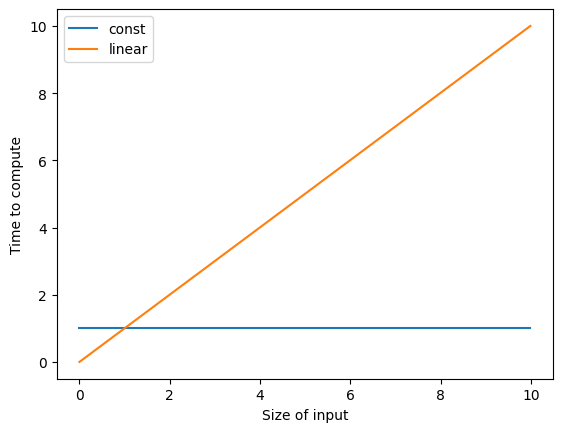
\includegraphics[width=\columnwidth]{images/complex1.png}
    \end{columns}
\end{frame}

\begin{frame}{Complexity}
    \begin{columns}
    \column{0.3\textwidth}
    \begin{itemize}
        \item Check odd or even\\
        \item Add two numbers \\
        \item Multiply two numbers \\
    \end{itemize}
    \column{0.7\textwidth}
    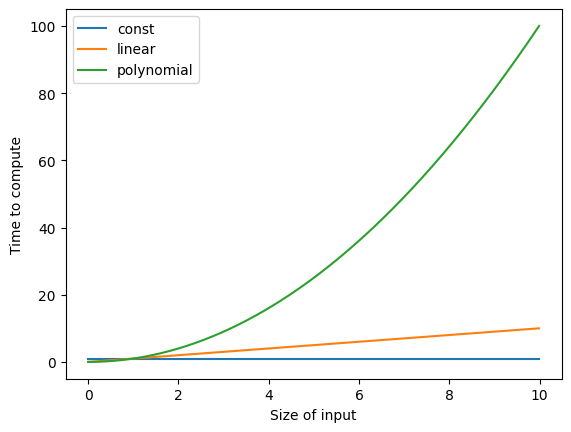
\includegraphics[width=\columnwidth]{images/complex2.png}
    \end{columns}
\end{frame}

\begin{frame}{Complexity}
    \begin{columns}
    \column{0.3\textwidth}
    \begin{itemize}
        \item Check odd or even\\
        \item Add two numbers \\
        \item Multiply two numbers \\
        \item Factorise a number \\
    \end{itemize}
    \column{0.7\textwidth}
    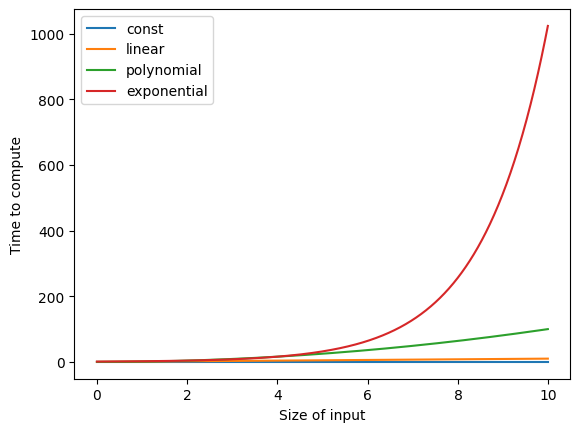
\includegraphics[width=\columnwidth]{images/complex3.png}
    \end{columns}
\end{frame}

\begin{frame}{Complexity}
    \begin{columns}
    \column{0.3\textwidth}
    \begin{itemize}
        \item Check odd or even \\
        \item Add two numbers \\
        \item Multiply two numbers \\
        \item Factorise a number \\
        \item Find the quickest route for a delivery truck
    \end{itemize}
    \column{0.7\textwidth}
    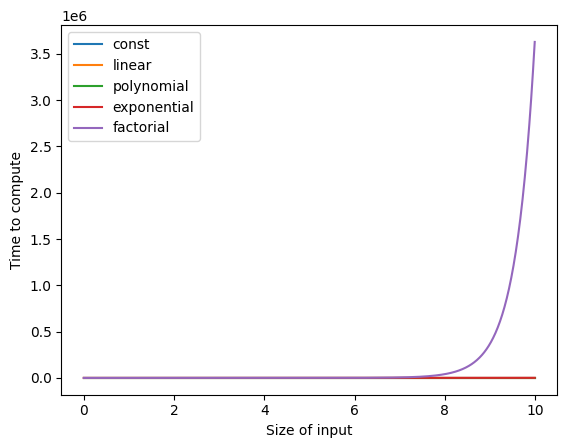
\includegraphics[width=\columnwidth]{images/complex4.png}
    \end{columns}
\end{frame}

\begin{frame}{Complexity}
    \begin{columns}
    \column{0.3\textwidth}
    \begin{itemize}
        \item Find the quickest route for a delivery truck \\
        \item Find all possible energy states of a molecule
    \end{itemize}
    \column{0.7\textwidth}
    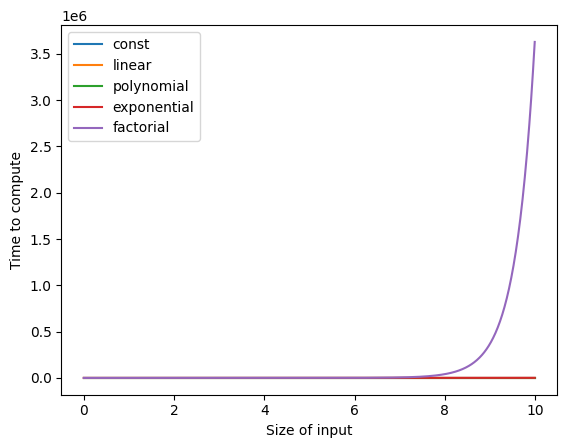
\includegraphics[width=\columnwidth]{images/complex4.png}
    \end{columns}
\end{frame}

\begin{frame}{Feynman}
    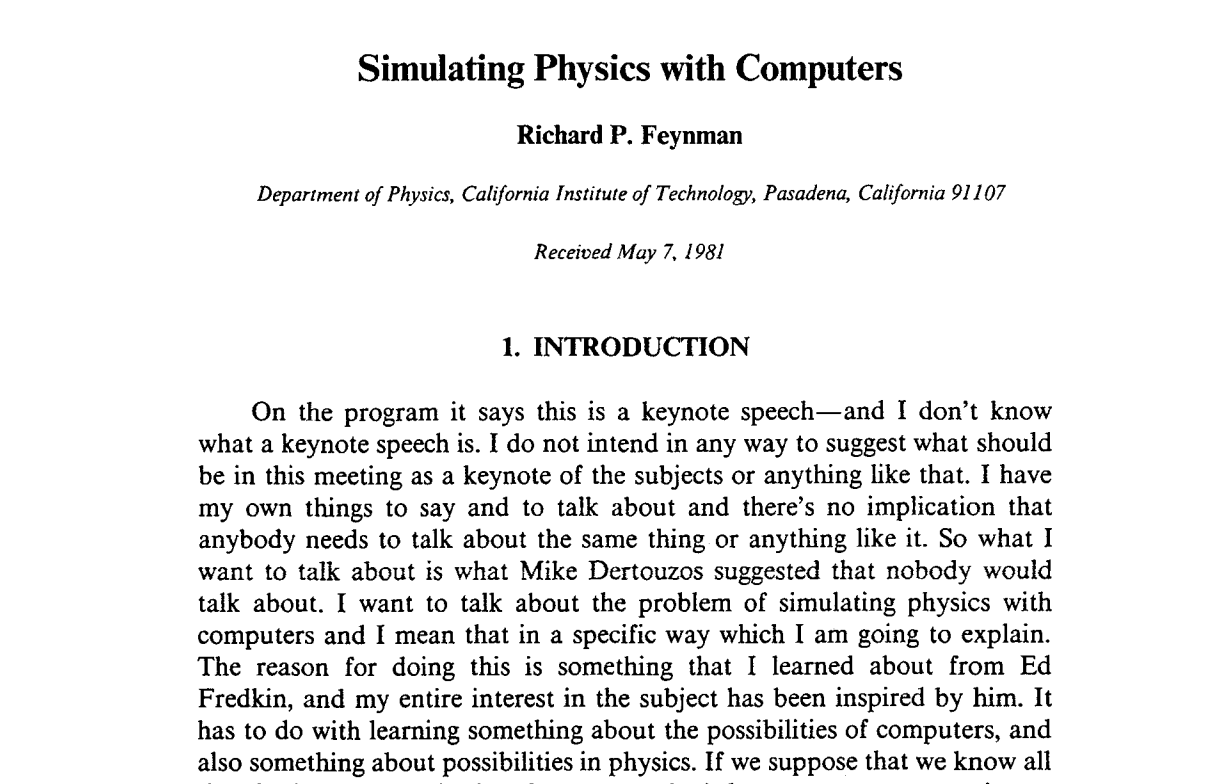
\includegraphics[width=\columnwidth]{images/feynman_paper.png}
\end{frame}

\begin{frame}{Uses for Quantum Computers}
    \begin{itemize}
        \item Design Pharmaceuticals
        \pause
        \item Save energy
        \pause
        \item Encryption / Decryption
        \pause
        \item Machine Learning
        \pause
        \item More we don't know yet!
    \end{itemize}
\end{frame}


%%%%%%%%%%%%%%%%%%%%%%%%%%%%%%%%%%%%%%%%%%%%%%%%%%%%%%%
% \section{Brief History of Quantum Mechanics}



%%%%%%%%%%%%%%%%%%%%%%%%%%%%%%%%%%%%%%%%%%%%%%%%%%%%%%%
\section{Computational Logic}

\begin{frame}<1>[label=whatdo]{What does a computer do?}
    We're going to approach quantum computing from the computing side, and add in quantum mechanics as we go.\vfill

    \begin{enumerate}
        \item<alert@1> Arithmetic / Logic
        \item<alert@2> Read / Write Memory
        \item<alert@3> Control Flow
    \end{enumerate}
\end{frame}

\begin{frame}{Logic Gates}
    \begin{columns}
        \column{0.3\textwidth}
        \centering
        NOT \\
        \begin{circuitikz}
	   \draw (0,0) node[not port] {};
        \end{circuitikz}        
        \column{0.3\textwidth}
        \centering
        AND \\
        \begin{circuitikz}
	   \draw (0,0) node[and port] {};
        \end{circuitikz}        
        \column{0.3\textwidth}
        \centering
        OR \\
        \begin{circuitikz}
	   \draw (0,0) node[or port] {};
        \end{circuitikz}    
        \end{columns}
\end{frame}

\begin{frame}{NOT Gate}
    \begin{columns}
        \column{0.5\textwidth}
        \centering
        \begin{circuitikz}
	   \draw (0,0) node[not port] (mynot) {}
            (mynot.in) node [anchor=east] {OFF}
            (mynot.out) node [anchor=west] {ON};
        \end{circuitikz}
        \column{0.5\textwidth}
        \centering
        \begin{circuitikz}
	   \draw (0,0) node[not port] (mynot) {}
            (mynot.in) node [anchor=east] {ON}
            (mynot.out) node [anchor=west] {OFF};     \end{circuitikz}
    \end{columns}
\end{frame}

\begin{frame}{NOT Gate}
    \begin{columns}
        \column{0.3\textwidth}
        \centering
        \begin{circuitikz}
	   \draw (0,0) node[not port] (mynot) {}
            (mynot.in) node [anchor=east] {False}
            (mynot.out) node [anchor=west] {True};
        \end{circuitikz}
        \column{0.3\textwidth}
        \centering
        \begin{circuitikz}
	   \draw (0,0) node[not port] (mynot) {}
            (mynot.in) node [anchor=east] {True}
            (mynot.out) node [anchor=west] {False};        \end{circuitikz}
    \end{columns}
\end{frame}

\begin{frame}{NOT Gate}
    \begin{columns}
        \column{0.3\textwidth}
        \centering
        \begin{circuitikz}
	   \draw (0,0) node[not port] (mynot) {}
            (mynot.in) node [anchor=east] {OFF}
            (mynot.out) node [anchor=west] {ON};
        \end{circuitikz} \\
        \vspace{1cm}
        \begin{circuitikz}
	   \draw (0,0) node[not port] (mynot) {}
            (mynot.in) node [anchor=east] {0}
            (mynot.out) node [anchor=west] {1};
        \end{circuitikz}
        \column{0.3\textwidth}
        \centering
        \begin{circuitikz}
	   \draw (0,0) node[not port] (mynot) {}
            (mynot.in) node [anchor=east] {ON}
            (mynot.out) node [anchor=west] {OFF};
        \end{circuitikz}\\
        \vspace{1cm}
        \begin{circuitikz}
	   \draw (0,0) node[not port] (mynot) {}
            (mynot.in) node [anchor=east] {1}
            (mynot.out) node [anchor=west] {0};
        \end{circuitikz}
    \end{columns}
\end{frame}

\begin{frame}{AND Gate}
    \begin{columns}
        \column{0.3\textwidth}
        \centering
        \begin{circuitikz}
	   \draw (0,0) node[and port] (myand) {}
            (myand.in 1) node [anchor=east] {0}
            (myand.in 2) node [anchor=east] {0}
            (myand.out) node [anchor=west] {0};
        \end{circuitikz} \\
        \vspace{1cm}
        \begin{circuitikz}
	   \draw (0,0) node[and port] (myand) {}
            (myand.in 1) node [anchor=east] {0}
            (myand.in 2) node [anchor=east] {1}
            (myand.out) node [anchor=west] {0};
        \end{circuitikz} \\
        \column{0.3\textwidth}
        \centering
        \begin{circuitikz}
	   \draw (0,0) node[and port] (myand) {}
            (myand.in 1) node [anchor=east] {1}
            (myand.in 2) node [anchor=east] {0}
            (myand.out) node [anchor=west] {0};
        \end{circuitikz} \\
        \vspace{1cm}
        \begin{circuitikz}
	   \draw (0,0) node[and port] (myand) {}
            (myand.in 1) node [anchor=east] {1}
            (myand.in 2) node [anchor=east] {1}
            (myand.out) node [anchor=west] {1};
        \end{circuitikz} \\
    \end{columns}
\end{frame}

\begin{frame}{OR Gate}
    \begin{columns}
        \column{0.3\textwidth}
        \centering
        \begin{circuitikz}
	   \draw (0,0) node[or port] (myor) {}
            (myor.in 1) node [anchor=east] {0}
            (myor.in 2) node [anchor=east] {0}
            (myor.out) node [anchor=west] {0};
        \end{circuitikz} \\
        \vspace{1cm}
        \begin{circuitikz}
	   \draw (0,0) node[or port] (myor) {}
            (myor.in 1) node [anchor=east] {0}
            (myor.in 2) node [anchor=east] {1}
            (myor.out) node [anchor=west] {1};
        \end{circuitikz} \\
        \column{0.3\textwidth}
        \centering
        \begin{circuitikz}
	   \draw (0,0) node[or port] (myor) {}
            (myor.in 1) node [anchor=east] {1}
            (myor.in 2) node [anchor=east] {0}
            (myor.out) node [anchor=west] {1};
        \end{circuitikz} \\
        \vspace{1cm}
        \begin{circuitikz}
	   \draw (0,0) node[or port] (myor) {}
            (myor.in 1) node [anchor=east] {1}
            (myor.in 2) node [anchor=east] {1}
            (myor.out) node [anchor=west] {1};
        \end{circuitikz} \\
    \end{columns}
\end{frame}

\begin{frame}{Combining gates}
    We can combine gates into circuits.\vfill
    \centering
    \begin{circuitikz}
        \draw 
        (0,0) node[not port] (mynot0) {}
        (2,0) node[not port] (mynot1) {}
        (mynot0.out) -| (mynot1.in 1);
    \end{circuitikz}\vfill
    \pause
    \begin{circuitikz}
        \draw 
        (0,0) node[and port] (myand1) {}
        (1,0) node[not port] (mynot1) {}
        (myand1.out) -| (mynot1.in 1);
    \end{circuitikz}\vfill
    
\end{frame}

\begin{frame}{FANOUT}
    We can split the wire in two.\vfill
        \centering
        \begin{circuitikz}\draw
            (3,0) node[and port] (mynand2) {}
            (1,0) -| (mynand2.in 1)
            (1,0) -| (mynand2.in 2);
        \end{circuitikz}\vfill
        \begin{circuitikz}\draw
            (3,0) node[or port] (mynand2) {}
            (1,0) -| (mynand2.in 1)
            (1,0) -| (mynand2.in 2);
        \end{circuitikz}\vfill
\end{frame}

\begin{frame}{FANOUT}
    This allows us to share inputs between gates.\vfill
    \centering
        \begin{circuitikz}\draw
            (2,1) node[and port] (myand) {}
            (0,0) -| (myand.in 2)
            (0,1.5) -| (myand.in 1)
            (2,-1) node[or port] (myor) {}
            (0,0) -| (myor.in 1)
            (0,-1.5) -| (myor.in 2);
        \end{circuitikz}\vfill
\end{frame}

\begin{frame}{First Circuit}
\centering
\begin{circuitikz} \draw
(0,1) node[or port] (myor1) {}
    (myor1.in 1) node [anchor=east] {0}
    (myor1.in 2) node [anchor=east] {1}
(-0.5,-1) node[not port] (mynot1) {}
    (mynot1.in) node [anchor=east] {1}
(2,0) node[and port] (myand1) {}
    (myand1.out) node [anchor=west] {X}
    (myor1.out) -| (myand1.in 1)
    (mynot1.out) -| (myand1.in 2);
\end{circuitikz}
\end{frame}

\begin{frame}{First Circuit}
\centering
\begin{circuitikz} \draw
(0,1) node[or port] (myor1) {}
    (myor1.in 1) node [anchor=east] {1}
    (myor1.in 2) node [anchor=east] {1}
(-0.5,-1) node[not port] (mynot1) {}
    (mynot1.in) node [anchor=east] {0}
(2,0) node[and port] (myand1) {}
    (myand1.out) node [anchor=west] {X}
    (myor1.out) -| (myand1.in 1)
    (mynot1.out) -| (myand1.in 2);
\end{circuitikz}
\end{frame}

\begin{frame}{Universality of NAND}
    \begin{columns}
    \column{0.5\textwidth}
    \centering
    \begin{circuitikz}
        \draw 
        (0,0) node[and port] (myand1) {}
        (1,0) node[not port] (mynot1) {}
        (myand1.out) -| (mynot1.in 1);
    \end{circuitikz}
    \column{0.5\textwidth}
    \centering
        \begin{circuitikz}
            \draw
            (0,0) node[nand port] {};
        \end{circuitikz}
    \end{columns}
    
    \begin{theorem}
        All logical operations can be completed with the NAND gate, they are said to be universal.
    \end{theorem}
    
    \vspace{1cm}
    
    Try to put these together to make something which behaves the same way as NOT, AND and OR gate.\footnote{(Hint: You can split lines or cross them over!)}
\end{frame}

\begin{frame}{Universality of NAND}
    \begin{columns}
        \column{0.5\textwidth}
        \centering
        \begin{circuitikz}
            \draw
            (0,0) node[not port] (mynot1) {};
        \end{circuitikz}
        \column{0.5\textwidth}
        \centering
        \begin{circuitikz}\draw
            (3,0) node[nand port] (mynand2) {}
            (1,0) -| (mynand2.in 1)
            (1,0) -| (mynand2.in 2);
        \end{circuitikz}
    \end{columns}
\end{frame}

\begin{frame}{Universality of NAND}
    \begin{columns}
        \column{0.5\textwidth}
        \centering
        \begin{circuitikz}
            \draw
            (0,0) node[and port] (mynot1) {};
        \end{circuitikz}
        \column{0.5\textwidth}
        \centering
        \begin{circuitikz}\draw
            (0,0) node[nand port] (mynand1) {}
            (2.5,0) node[nand port] (mynand2) {}
            (mynand1.out) -| (1,0)
            (1,0) -| (mynand2.in 1)
            (1,0) -| (mynand2.in 2);
        \end{circuitikz}
    \end{columns}
\end{frame}

\begin{frame}{Universality of NAND}
    \begin{columns}
        \column{0.5\textwidth}
        \centering
        \begin{circuitikz}
            \draw
            (0,0) node[or port] (mynot1) {};
        \end{circuitikz}
        \column{0.5\textwidth}
        \centering
        \begin{circuitikz}\draw
            (0,0) node[nand port] (mynand1) {}
            (0,2) node[nand port] (mynand3) {}
            (2,1) node[nand port] (mynand2) {}
            (-2,0) -| (mynand1.in 1)
            (-2,0) -| (mynand1.in 2)
            (-2,2) -| (mynand3.in 1)
            (-2,2) -| (mynand3.in 2)
            (mynand3.out) -| (mynand2.in 1)
            (mynand1.out) -| (mynand2.in 2);
        \end{circuitikz}
    \end{columns}
\end{frame}

\begin{frame}{States}
    For binary systems we can define two states of each input.\vfill
    \begin{columns}
        \column{0.5\textwidth}
        \centering
        OFF = $\ket{0}$
        \column{0.5\textwidth}
        \centering
        ON = $\ket{1}$
    \end{columns}\vfill
\end{frame}

\begin{frame}{Operators}
    Rather than draw the gate we can use its name, like we would for a function.\vfill
    \begin{columns}
        \column{0.5\textwidth}
        \centering
        \begin{circuitikz}
	   \draw (0,0) node[not port] (mynot) {}
            (mynot.in) node [anchor=east] {0}
            (mynot.out) node [anchor=west] {1};
        \end{circuitikz}
        \column{0.5\textwidth}
        \centering
        \begin{circuitikz}
	   \draw (0,0) node[not port] (mynot) {}
            (mynot.in) node [anchor=east] {1}
            (mynot.out) node [anchor=west] {0};
        \end{circuitikz}
    \end{columns}\vfill
    \vfill
    \begin{columns}
        \column{0.5\textwidth}
        \centering
        \begin{math}
            NOT\ket{0} = \ket{1}
        \end{math}
        \column{0.5\textwidth}
        \centering
        \begin{math}
            NOT\ket{1} = \ket{0}
        \end{math}
    \end{columns}\vfill
    \pause
    We can go one step further and use a symbol.\vfill

    \begin{columns}
        \column{0.5\textwidth}
        \centering
        \begin{math}
            \hat{N}\ket{0} = \ket{1}
        \end{math}
        \column{0.5\textwidth}
        \centering
        \begin{math}
            \hat{N}\ket{1} = \ket{0}
        \end{math}
    \end{columns}\vfill
    \pause
    Gates are represented by symbols with hats, called \emph{operators}.
\end{frame}

\begin{frame}<1>[label=multiop]{Multi-bit Operators}
    We can apply multi-bit operators to multi-bit states.\vfill
    \begin{columns}
    \column{0.5\textwidth}
    \centering
    \only<1>{
    \begin{tabular}{r}
    % \begin{math}
    %     \hat{A}\ket{xy} = \ket{z}
    % \end{math}\\
    \begin{math}
        \hat{A}\ket{00} = \ket{0}
    \end{math}\\
    \begin{math}
        \hat{A}\ket{01} = \ket{0}
    \end{math}\\
    \begin{math}
        \hat{A}\ket{10} = \ket{0}
    \end{math}\\
    \begin{math}
        \hat{A}\ket{11} = \ket{1}
    \end{math}
    \end{tabular}
    }
    \only<2>{
    \begin{tabular}{r}
    \begin{math}
        \hat{O}\ket{00} = \ket{0}
    \end{math}\\
    \begin{math}
        \hat{O}\ket{01} = \ket{1}
    \end{math}\\
    \begin{math}
        \hat{O}\ket{10} = \ket{1}
    \end{math}\\
    \begin{math}
        \hat{O}\ket{11} = \ket{1}
    \end{math}
    \end{tabular}
    }
    \column{0.5\textwidth}
    \centering
    \only<1>{
    \begin{circuitikz}\draw
        (0,0) node [and port] {};
    \end{circuitikz}
    }
    \only<2>{
    \begin{circuitikz}\draw
        (0,0) node [or port] {};
    \end{circuitikz}
    }
    \end{columns}
\end{frame}
\againframe<2>{multiop}


\begin{frame}{Rules for Operators}

    Operators act to their right.
    \vfill

    \centering
    \begin{math}
        \hat{N}\ket{0} = \ket{1}
    \end{math}\vfill
    \pause
    \begin{math}
        \hat{N}\hat{A}\ket{11} = \hat{N}\bigg(\hat{A}\ket{11}\bigg) = \hat{N}\ket{1} = \ket{0}
    \end{math}
\end{frame}

\begin{frame}{Rules for Operators}

    Operators only act on states with the correct size of input
    \vfill

    \centering
    \begin{math}
        \hat{A}\ket{0} = 0
    \end{math}\vfill
    \begin{math}
        \hat{N}\ket{11} = 0
    \end{math}
\vfill

Note that this is $0$ and not a state at all!
\end{frame}

\begin{frame}{Rules for Operators}

    Operators can be applied multiple times.
    \vfill

\centering
    \begin{math}
        \hat{N}\hat{N}\ket{1} = \hat{N}\ket{0}= \ket{1}
    \end{math}
\end{frame}

\begin{frame}{Identity Operator}
    We define the Identity Operator $\hat{\mathbb{I}}$ which does nothing to change the state.
    \vfill
    \centering
    \begin{columns}
    \column{0.3\textwidth}
    \centering
    \begin{math}
        \hat{\mathbb{I}}\ket{0}
        = \ket{0}
    \end{math}
    \column{0.3\textwidth}
    \centering
    \begin{math}
        \hat{\mathbb{I}}\ket{1}
        = \ket{1}
    \end{math}
    \end{columns}\vfill
    This is equivalent to a wire in our circuit.\vfill
    \begin{center}
        \begin{circuitikz}\draw
            (0,0) -| (2,0)
            (0,0) node [anchor=east] {0}
            (2,0) node [anchor=west] {0};
        \end{circuitikz}
    \end{center}

\end{frame}

\begin{frame}{Identity Operator}
    This allows us write about operators independent of states.
    \vfill

\centering
    \begin{math}
        \hat{N}\hat{N}\ket{0} = \hat{N}\ket{1} = \hat{\mathbb{I}}\ket{0}
    \end{math}\vfill
    \begin{math}
        \hat{N}\hat{N}\ket{1} = \hat{N}\ket{0} = \hat{\mathbb{I}}\ket{1}
    \end{math}\vfill
    \begin{math}
        \hat{N}\hat{N} = \hat{\mathbb{I}}
    \end{math}
\end{frame}

\begin{frame}{States}
    For binary systems we can define two states of each input.\vfill
    \begin{columns}
        \column{0.5\textwidth}
        \centering
        OFF = $\ket{0}$
        \column{0.5\textwidth}
        \centering
        ON = $\ket{1}$
    \end{columns}\vfill    
    \pause
    The states have a property called the \textbf{inner product}.\vfill
    \pause
    \begin{center}
    \begin{math}
        \braket{0}{0} = \braket{1}{1} = 1
    \end{math}\vfill
    \begin{math}
        \braket{0}{1} = \braket{1}{0} = 0
    \end{math}\vfill
    \end{center}
    \pause
    This is essentially the question 'are these the same state?'
\end{frame}

\begin{frame}{Multi-bit States}
To combine single bit states into larger sizes we use a \emph{tensor product}.\footnote{We don't want to multiply the values, just list them in order!}\vfill

\centering
\begin{math}
    \ket{x} \otimes \ket{y}
    = \ket{xy}
\end{math}\vfill
    e.g.
\begin{math}
    \ket{0} \otimes \ket{1}
    = \ket{01}
\end{math}\vfill
\end{frame}

\begin{frame}{Multi-bit Inner Product}
We can work out the inner product using the single bit definitions.\vfill
\begin{center}
\begin{math}
    \bra{\textcolor{red}{a}\textcolor{blue}{b}}\ket{\textcolor{red}{c}\textcolor{blue}{d}}
\end{math}\vfill
\begin{math}
    =(\textcolor{red}{\bra{a}} \otimes \textcolor{blue}{\bra{b}})(\textcolor{red}{\ket{c}} \otimes \textcolor{blue}{\ket{d}})
\end{math}\vfill
\begin{math}
    =\textcolor{red}{\braket{a}{c}} \otimes \textcolor{blue}{\braket{b}{d}}
\end{math}\vfill
\end{center}
\pause
\begin{columns}
    \column{0.5\textwidth}
    \centering
    Similar states give 1:\\
    \begin{math}
        \braket{00}{00} = 1
    \end{math}
    \column{0.5\textwidth}
    \centering
    Different states give 0:\\
    \begin{math}
        \braket{00}{11} = 0
    \end{math}\\
    \begin{math}
        \braket{01}{11} = 0
    \end{math}\\
    \begin{math}
        \braket{10}{11} = 0
    \end{math}
    \end{columns}
\end{frame}

\begin{frame}{Rules for Operators}

However, we can use the tensor product to make larger operators.
    \vfill

    \centering
    \begin{math}
    \hat{\mathbb{I}}\otimes\hat{N}\ket{11} = (\hat{\mathbb{I}}\otimes\hat{N})(\ket{1}\otimes\ket{1})
    \end{math}\vfill
    \begin{math}
    = \hat{\mathbb{I}}\ket{1}\otimes\hat{N}\ket{1}
    \end{math}\vfill
    \begin{math}
    = \ket{1}\otimes\ket{0}
    \end{math}\vfill
    \begin{math}
    = \ket{10}
    \end{math}
\vfill

Similarly $(\hat{N}\otimes\hat{\mathbb{I}})\ket{11}=\ket{01}$ 
and $(\hat{N}\otimes\hat{N})\ket{11}=\ket{00}$
\end{frame}

\begin{frame}{Outer Product}
    So far we've learned the \textbf{tensor product}\vfill
    \begin{center}
        \begin{math}
            \ket{0} \otimes \ket{1} = \ket{01}
        \end{math}
    \end{center}\vfill
    \pause
    and the \textbf{inner product}\vfill
    \begin{center}
    \begin{math}
        \braket{0}{1} = 0
    \end{math}\vfill
    \end{center}
    \pause
    Can you guess what an \textbf{outer product} looks like?
    \vfill
    \pause
    \begin{center}
        \begin{math}
            \ket{0}\bra{1}
        \end{math}        
    \end{center}
\end{frame}

\begin{frame}{Outer Product}
    The outer product can be used to change a state. We start with $\ket{1}$.\vfill
    \begin{center}
        \begin{math}
            \ket{0}\bra{1} \ \ket{1}
        \end{math}\vfill
        \pause
        \begin{math}
            =\ket{0}\textcolor{red}{\bra{1}\ket{1}}
        \end{math}\vfill
        \pause
        \begin{math}
            =\ket{0}\times\textcolor{red}{1}
        \end{math}\vfill
    \end{center}
    \pause
    The state has been changed from $\ket{1}$ to $\ket{0}$!\vfill
    \begin{center}
        \begin{math}
            \ket{OUT}\bra{IN}
        \end{math}
    \end{center}
\end{frame}

\begin{frame}{Operators from Outer Products}
    We already saw that $\ket{0}\bra{1}$ changed 1 to 0.\vfill
    $\ket{1}\bra{0}$ does the opposite, it changes 0 to 1.\vfill
    \pause
    These are the conditions for the NOT gate and $\hat{N}$ operator.\vfill
    \centering
        \begin{math}
            \hat{N} = \ket{0}\bra{1} + \ket{1}\bra{0}
        \end{math}
\end{frame}

\begin{frame}{Operators from Outer Products}
    Lets see how he $\hat{N}$ operator works.\vfill
    \begin{center}
        \begin{math}
            \hat{N} = \ket{0}\bra{1} + \ket{1}\bra{0}
        \end{math}
        \vfill
        \begin{math}
            \hat{N}\ket{0} = (\ket{0}\bra{1} + \ket{1}\bra{0})\ket{0}\\
        \end{math}
        \pause
        \vfill
        \begin{math}
            \hat{N}\ket{0} = \ket{0}\textcolor{red}{\bra{1}\ket{0}} + \ket{1}\textcolor{red}{\bra{0}\ket{0}}
        \end{math}
        \pause
        \vfill
        \begin{math}
            \hat{N} \ket{0} = \ket{0}\times \textcolor{red}{0} + \ket{1} \times \textcolor{red}{1}
        \end{math}
        \pause
        \vfill
        \begin{math}
            \hat{N}\ket{0} = \ket{1}
        \end{math}
        
    \end{center}
\end{frame}

\begin{frame}{The AND Operator}
    Lets build up the $\hat{A}$ operator.\vfill
    \begin{center}
        
    \begin{tabular}{| c | c | c |}
        \hline
         Input & Output & Outer Product \\
         \hline
         $\ket{00}$ & $\ket{0}$ & $\ket{0}\bra{00}$\\
         \pause
         $\ket{01}$ & $\ket{0}$ & $\ket{0}\bra{01}$\\
         \pause
         $\ket{10}$ & $\ket{0}$ & $\ket{0}\bra{10}$\\
         \pause
         $\ket{11}$ & $\ket{1}$ & $\ket{1}\bra{11}$\\
         \hline
    \end{tabular}
    \vfill
    \pause
    \begin{math}
        \hat{A} = \ket{0}\bra{00} + \ket{0}\bra{01} + \ket{0}\bra{10} + \ket{1}\bra{11}
    \end{math}
    \end{center}
    \pause
    \vfill
    Notice that the states on the right have two bits but the states on the left only have one!
    
\end{frame}

\begin{frame}{The OR Operator}
    Lets build up the $\hat{O}$ operator.\vfill
    \begin{center}
        
    \begin{tabular}{| c | c | c |}
        \hline
         Input & Output & Outer Product \\
         \hline
         $\ket{00}$ & $\ket{0}$ & $\ket{0}\bra{00}$\\
         $\ket{01}$ & $\ket{1}$ & $\ket{1}\bra{01}$\\
         $\ket{10}$ & $\ket{1}$ & $\ket{1}\bra{10}$\\
         $\ket{11}$ & $\ket{1}$ & $\ket{1}\bra{11}$\\
         \hline
    \end{tabular}
    \vfill
    \begin{math}
        \hat{O} = \ket{0}\bra{00} + \ket{1}\bra{01} + \ket{1}\bra{10} + \ket{1}\bra{11}
    \end{math}
    \end{center}
\end{frame}


%%%%%%%%%%%%%%%%%%%%%%%%%%%%%%%%%%%%%%%%%%%%%%%%%%%%%%%
\section{Quantum States}

\begin{frame}<1>[label=postulates]{Postulates of QM}
    \begin{enumerate}
        \item<alert@1> State Vector
        \item<alert@2> Time Evolution
        \item<alert@3> Measurements
        \item<alert@4> Composite Systems
    \end{enumerate}
    
\end{frame}

\begin{frame}{Postulates of QM}
\begin{block}{Postulate 1}
Any isolated physical system is completely described by a state vector.
\end{block}
\vfill
A two state quantum system is called a \textbf{Qubit}.
\vfill
\centering
\begin{math}
    \ket{\Psi} = \alpha\ket{0} + \beta\ket{1}
\end{math}\vfill

Where $\alpha, \beta \in \mathbb{C}$ (they are complex numbers)
\footnote{where $\chi=a+ib$ is a complex number, $\chi^*=a-ib$.}
\vfill
\pause
\begin{math}
    \bra{\Psi} = \bra{0}\alpha^* + \bra{1}\beta^*
\end{math}
\vfill
\pause
\begin{math}
    \braket{\Psi}{\Psi} = \abs{\alpha}^2\braket{0}{0} + \alpha^*\beta\textcolor{red}{\braket{0}{1}} + \alpha\beta^*\textcolor{red}{\braket{1}{0}} + \abs{\beta}^2\braket{1}{1}
\end{math}\vfill\pause
\begin{math}
    1 = \abs{\alpha}^2 + \abs{\beta}^2
\end{math}\vfill
\end{frame}

\begin{frame}{Inner Product of Different States}
    Because we have amplitudes for each state $\ket{0}$ and $\ket{1}$ the inner products of two quantum states have values between 0 and 1.
    \begin{center}
        \begin{math}
            \ket{\Psi} = \alpha\ket{0} + \beta\ket{1}
        \end{math}\\
        \begin{math}
            \ket{\Phi} = \gamma\ket{0} + \delta\ket{1}
        \end{math}
        \vfill
        \begin{math}
            \braket{\Psi}{\Phi} = \alpha^*\gamma\braket{0}{0} + \beta^*\delta\braket{1}{1}
        \end{math}\vfill
        \begin{math}
            \braket{\Psi}{\Phi} = \alpha^*\gamma + \beta^*\delta
        \end{math}\vfill
        \begin{math}
            0 \le \braket{\Psi}{\Phi} \le 1
        \end{math}\vfill
    
    \end{center}
    
\end{frame}

\begin{frame}[label=p1]{Postulates of QM}
\begin{block}{Postulate 1}
Any isolated physical system is completely described by a state vector.
\end{block}\vfill
This is true not just for qubits, but for any size of quantum system.
\vfill
\centering
\begin{math}
    \ket{\Psi} = c_0\ket{\psi_0} + c_1\ket{\psi_1} + \dots + c_n\ket{\psi_n}
\end{math}\vfill

Where $\{c_0, c_1, \dots, c_n\} \in \mathbb{C}$\vfill

\begin{math}
    \abs{c_0}^2 + \abs{c_1}^2 + \dots + \abs{c_n}^2 = 1
\end{math}\vfill
\end{frame}
\againframe<2>{postulates}

\begin{frame}{Postulates of QM}
\begin{block}{Postulate 2}
    Evolution of a closed system is by \emph{unitary transformation}.
\end{block}\vfill

Unitary here means that the inner product $\braket{\Psi}{\Psi}$ is unchanged.\vfill
\centering
\begin{math}
    \hat{U}\ket{\Psi} = \ket{\Phi}
\end{math}\vfill
\begin{math}
    \braket{\Phi}{\Phi} = 1
\end{math}

\end{frame}
\againframe<3>{postulates}

\begin{frame}{Postulates of QM}
\begin{block}{Postulate 3}
    Measurements of quantum systems project the system onto one of its states.
\end{block}\vfill
For a single qubit state $\ket{\Psi} = \alpha\ket{0} + \beta\ket{1}$, a measurement of the qubit will transform it into the state $\ket{0}$ with probability $\abs{\alpha}^2$ or $\ket{1}$ with probability $\abs{\beta}^2$.

\end{frame}
\againframe<4>{postulates}

\begin{frame}{Postulates of QM}
\begin{block}{Postulate 4}
    The state vector of a composite system is the tensor product of the component systems state vectors.
\end{block}\vfill
\centering
\begin{math}    
\ket{\Psi} = \alpha\ket{0} + \beta\ket{1}
\end{math} \vfill
\begin{math}    
\ket{\Phi} = \gamma\ket{0} + \delta\ket{1}
\end{math}
\vfill
\begin{math}
    \ket{\Psi} \otimes \ket{\Phi} = \alpha\gamma\ket{00} + \alpha\delta\ket{01} + \beta\gamma\ket{10} + \beta\delta\ket{11}
\end{math}\vfill
% \begin{math}
%     \ket{\Psi} \otimes \ket{\Phi} = 
%     \begin{pmatrix}
%         \alpha \\ \beta
%     \end{pmatrix}
%     \otimes
%     \begin{pmatrix}
%         \gamma \\ \delta
%     \end{pmatrix}
%     =
%     \begin{pmatrix}
%         \alpha\gamma \\ \alpha\delta \\ \beta\gamma \\ \beta\delta
%     \end{pmatrix}
% \end{math}
\end{frame}

\begin{frame}{Quantum Entanglement}
    \begin{definition}
    To objects are entangled when their joint state $\ket{\Psi}$ cannot be expressed as the product of two states $\ket{\psi}\otimes\ket{\psi}$.
    \end{definition}
    \vfill
    \begin{center}
        \begin{math}
            \ket{\Psi} \ne \ket{\psi}\otimes\ket{\psi}
        \end{math}
    \end{center}
    \pause
    \begin{block}{Exercise}
    Show that the state $\ket{\Psi} = \frac{1}{\sqrt{2}}\ket{00} + \frac{1}{\sqrt{2}}\ket{11}$ is entangled by proving there are no values of of $\alpha_0, \alpha_1, \beta_0, \beta_1$ such that:\vfill
    \centering
    \begin{math}
        \ket{\Psi} = (\alpha_0\ket{0} + \beta_0\ket{1})(\alpha_1\ket{0} + \beta_1\ket{1})
    \end{math}\vfill
    \end{block}
\end{frame}

% \begin{frame}<1>[label=pnot]{Probabilistic Not}
%     So far we've made circuits assuming we know for sure what the state is. 
%         \vfill
%         \centering
%         \begin{circuitikz}
% 	       \draw
%             (0,0) node[not port] (mynot) {}
%             (mynot.in) node [anchor=east] {0}
%             (mynot.out) node [anchor=west] {1};
%         \end{circuitikz}\vfill
%         \pause
%         What if we only knew with some probability whether an input was in state $\ket{0}$ or $\ket{1}$?
%         \vfill
%         \only<1>{
%         \begin{circuitikz}
% 	       \draw
%             (0,0) node[not port] (mynot) {}
%             (mynot.in) node [anchor=east] {0.25}
%             (mynot.out) node [anchor=west] {?}
%             ;
%         \end{circuitikz}}
%         \only<2>{
%         \begin{circuitikz}
% 	       \draw
%             (0,0) node[not port] (mynot) {}
%             (mynot.in) node [anchor=east] {0.25}
%             (mynot.out) node [anchor=west] {0.75}
%             ;
%         \end{circuitikz}}
% \end{frame}
% \againframe<2>{pnot}

% \begin{frame}{Probabilistic State}
%     If we define the state to be $\ket{s}$ to be $\ket{0}$ with probability $p_0$ and $\ket{1}$ with probability $p_1$.\vfill
%     \begin{center}
%         \begin{math}
%             \ket{s} = p_0\ket{0} + p_1\ket{1}
%         \end{math}\vfill
%     \end{center}
%     \vfill
%     What rules do we need for $p_0$ and $p_1$?
% \end{frame}

% \begin{frame}{Total Probability}
%     Probabilities need to add up to 1.\vfill
%     \begin{columns}
%         \column{0.5\textwidth}
%         \centering
%         Coin Flip\vfill
%         \begin{math}
%             Prob({HEAD}) = 0.5 
%         \end{math}\vfill
%         \begin{math}
%             Prob({TAIL}) = 0.5 
%         \end{math}\vfill
%         \column{0.5\textwidth}
%         \centering
%         Dice Roll\vfill
%         \begin{math}
%             Prob(1) = \frac{1}{6} 
%         \end{math}\vfill
%         \begin{math}
%             Prob(2) = \frac{1}{6} 
%         \end{math}\vfill
%         \dots\vfill
%         \begin{math}
%             Prob(6) = \frac{1}{6} 
%         \end{math}\vfill
%     \end{columns}
%     Our total probabilities must add up to 1!
% \end{frame}

% \begin{frame}{Probabilistic Not}
%     Let's apply the NOT gate to $\ket{s}$.\vfill
%     \centering
%         \begin{math}
%             \hat{N}\ket{s} = \hat{N}(p_0\ket{0} + p_1\ket{1})
%         \end{math}\vfill
%         \begin{math}
%             = p_0\hat{N}\ket{0} + p_1\hat{N}\ket{1}
%         \end{math}\vfill
%         \begin{math}
%             = p_0\ket{1} + p_1\ket{0}
%         \end{math}
%         \vfill
%         % \pause
%         % \begin{math}
%         %     \hat{N}\ket{s} = 
%         %     \begin{pmatrix}
%         %         0 & 1 \\ 1 & 0
%         %     \end{pmatrix}
%         %     \begin{pmatrix}
%         %         p_0 \\ p_1
%         %     \end{pmatrix}
%         % \end{math}\vfill
%         % \begin{math}
%         %     = 
%         %     \begin{pmatrix}
%         %         p_1 \\ p_0
%         %     \end{pmatrix}
%         % \end{math}\vfill

% \end{frame}

% \begin{frame}{Probabilistic Computing}
%     Previously we've only used states 0 and 1.\vfill
%     \begin{columns}
%         \column{0.5\textwidth}
%         \centering
%         \begin{math}
%             \ket{0} = \begin{pmatrix}
%                 1 \\ 0
%             \end{pmatrix}
%         \end{math}
%         \column{0.4\textwidth}
%         \centering
%         \begin{math}
%             \ket{1} = \begin{pmatrix}
%                 0 \\ 1
%             \end{pmatrix}
%         \end{math}
%     \end{columns}\vfill
%     \pause
%     But we saw that we can use vectors for arbitrary numbers.\vfill
%     Imagine we didn't know whether we had state $\ket{0}$ or $\ket{1}$.
% \end{frame}

% \begin{frame}{Probabilistic Logic}
%     We could create a state which is a combination of the two of these.\vfill
%     \begin{center}
%         \begin{math}
%             \ket{s} = p_0\ket{0} + p_1\ket{1}
%         \end{math}\vfill
%         \begin{math}
%             \ket{s} =
%             p_0\begin{pmatrix}
%                 1 \\ 0
%             \end{pmatrix}
%             +
%             p_1\begin{pmatrix}
%                 0 \\ 1
%             \end{pmatrix}
%         \end{math}\vfill
%         \begin{math}
%             \ket{s} =
%             \begin{pmatrix}
%                 p_0 \\ p_1
%             \end{pmatrix}
%         \end{math}
%     \end{center}
%     \vfill
%     \pause
%     Where $0\le p \le 1$.
%     \note{What rules do we need to have have for p_0 and p_1?}
% \end{frame}


% \begin{frame}{Probabilistic Not}
%     Let's apply the NOT gate to $\ket{s}$.\vfill
%     \centering
%         \begin{math}
%             \hat{N}\ket{s} = \hat{N}(p_0\ket{0} + p_1\ket{1})
%         \end{math}\vfill
%         \begin{math}
%             = p_0\hat{N}\ket{0} + p_1\hat{N}\ket{1}
%         \end{math}\vfill
%         \begin{math}
%             = p_0\ket{1} + p_1\ket{0}
%         \end{math}
%         \vfill
%         \pause
%         \begin{math}
%             \hat{N}\ket{s} = 
%             \begin{pmatrix}
%                 0 & 1 \\ 1 & 0
%             \end{pmatrix}
%             \begin{pmatrix}
%                 p_0 \\ p_1
%             \end{pmatrix}
%         \end{math}\vfill
%         \begin{math}
%             = 
%             \begin{pmatrix}
%                 p_1 \\ p_0
%             \end{pmatrix}
%         \end{math}\vfill

% \end{frame}


% \begin{frame}{Joint Probability}
%     The probability of two independent events happening is the product of their individual probabilities.\vfill
%     For instance, throwing two coins 'A' and 'B' will give heads with the probability:
%     \vfill
%     \centering
%     \begin{math}
%         Prob_{A,B}(HEAD,HEAD) = Prob_A(HEAD) * Prob_B(HEAD)
%     \end{math}\vfill
%     \begin{math}
%         = 0.5 * 0.5 = 0.25
%     \end{math}
% \end{frame}

% \begin{frame}{Joint Probability}
%     More generally for two states:
%     \vfill
%     \centering
%     \begin{math}
%         \ket{s_1} = 
%         \begin{pmatrix}
%             p_0 \\ p_1
%         \end{pmatrix}
%     \end{math}\vfill
%     \begin{math}
%         \ket{s_2} = 
%         \begin{pmatrix}
%             q_0 \\ q_1
%         \end{pmatrix}
%     \end{math}\vfill
%     \begin{math}
%         \ket{s_1} \otimes \ket{s_2} = 
%         \begin{pmatrix}
%             p_0 \\ p_1
%         \end{pmatrix}
%         \otimes
%         \begin{pmatrix}
%             q_0 \\ q_1
%         \end{pmatrix}
%         =         
%         \begin{pmatrix}
%             p_0 q_0 \\ p_0q_1 \\ p_1q_0 \\ p_1q_1
%         \end{pmatrix}
%     \end{math}\vfill
%     \pause
% \begin{block}{Exercise}
%     Try applying $A$ and $O$ in matrix form to this state, what is the probability of $\ket{0}$?
% \end{block}
% \end{frame}


\begin{frame}{Number of Parameters}
    In the example where we combine two qubits\vfill
    \begin{center}
        \begin{math}
            \ket{\Psi} \otimes \ket{\Phi} = \alpha\gamma\ket{00} + \alpha\delta\ket{01} + \beta\gamma\ket{10} + \beta\delta\ket{11}
        \end{math}
    \end{center}
    \vfill
    We need 4 terms to describe the state. If we take the tensor product with another qubit:\vfill
    \pause
    \begin{center}
        \begin{math}    
            \ket{\chi} = \nu\ket{0} + \mu\ket{1}
        \end{math}
    \end{center}
    \vfill
    \begin{center}
        \pause
        \begin{math}
            \ket{\Psi} \otimes \ket{\Phi} \otimes \ket{\chi} = \nu\alpha\gamma\ket{000} + \nu\alpha\delta\ket{001} + \nu\beta\gamma\ket{010} + \nu\beta\delta\ket{011} + \mu\alpha\gamma\ket{100} + \mu\alpha\delta\ket{101} + \mu\beta\gamma\ket{110} + \mu\beta\delta\ket{111}
        \end{math}
    \end{center}
    \vfill
    \pause
    Now there are 8 terms!\\
    Generally, the number of terms is $2^N$, where $N$ is the number of qubits.
\end{frame}

\begin{frame}{Too many states}
    The state/operator notation works great for logical circuits. Inputs and Output are states, and gates are operators which transform the states.\vfill

    It also works really well for representing quantum states.\vfill

    However, it gets a little hard to work with for larger states.
\end{frame}

\begin{frame}<1>[label=statevec]{State Vectors}
    We can handle complex states more easily if we switch to expressing states using vector notation.\\
    \vfill
    
    \centering
    \begin{columns}
        \column{0.5\textwidth}
        \centering
        \begin{math}
            \ket{0} = \begin{pmatrix}
                1 \\ 0
            \end{pmatrix}
        \end{math}
        \column{0.4\textwidth}
        \centering
        \begin{math}
            \ket{1} = \begin{pmatrix}
                0 \\ 1
            \end{pmatrix}
        \end{math}
    \end{columns}\vfill
    \only<2>{
    \begin{columns}
        \column{0.5\textwidth}
        \centering
        \begin{math}
            \bra{0} = \begin{pmatrix}
                1 & 0
            \end{pmatrix}
        \end{math}
        \column{0.4\textwidth}
        \centering
        \begin{math}
            \bra{1} = \begin{pmatrix}
                0 & 1
            \end{pmatrix}
        \end{math}
    \end{columns}
    }
\end{frame}

\begin{frame}{Vectors}
    Vectors are often used to point to a location in space.\\
    For instance, here's a representation of the vector $\begin{pmatrix}
        3 \\ 2
    \end{pmatrix}$
    \centering
    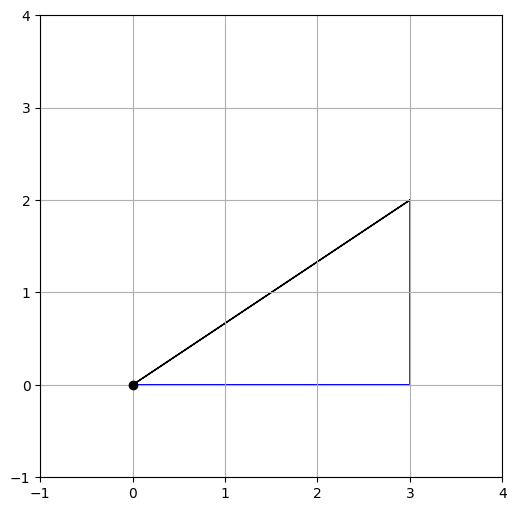
\includegraphics[scale=0.4]{images/vectorgrid.png}
\end{frame}


\begin{frame}{Bloch Sphere}
    Vectors can be thought of as arrows with a certain length and direction.\vfill
    Quantum states can be represented by a point on the \textbf{Bloch Sphere}.\vfill

    \begin{columns}
        \column{0.5\textwidth}
        \begin{figure}
            \centering
            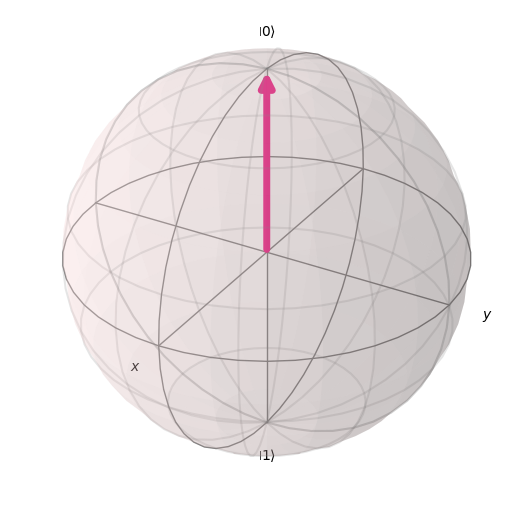
\includegraphics[width=0.8\columnwidth]{images/bloch+z.png}
            \caption{$\ket{\Psi}=\ket{0}$}
        \end{figure}
        \column{0.5\textwidth}
        \begin{figure}
            \centering
            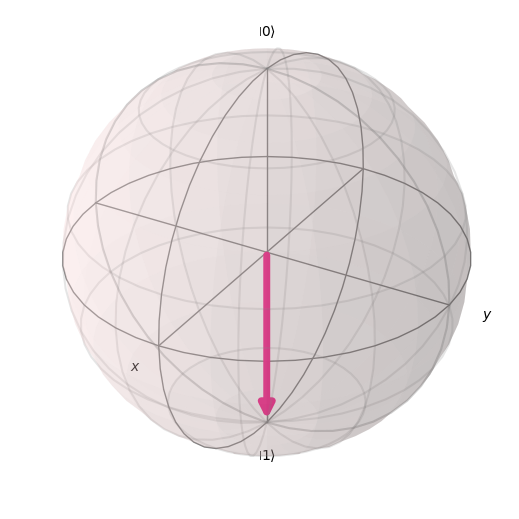
\includegraphics[width=0.8\columnwidth]{images/bloch-z.png}
            \caption{$\ket{\Psi}=\ket{1}$}
        \end{figure}
    \end{columns}
    
    We'll explore the the Bloch sphere in the practical parts of the day. 
\end{frame}

\begin{frame}[label=vectors]{Rules for Vectors}

    With two vectors $\ket{x} = \begin{pmatrix} a_0 \\ b_0 \end{pmatrix}$ and $\ket{y} = \begin{pmatrix} a_1 \\ b_1 \end{pmatrix}$, we define:\vfill

    \centering
    \begin{tabular}{l l}
        \textbf{Addition} & \\
        \begin{math}
            \ket{x}+\ket{y} = \begin{pmatrix}
                a_0+a_1 \\ b_0+b_1
            \end{pmatrix}
        \end{math} & \\[3ex]
        \textbf{Scalar Multiplication} & \textbf{Inner Product}\footnote{if $z=x+iy$ then $z^*=x-iy$} \\
               \begin{math}
            n * \ket{x} = \begin{pmatrix}
                n * a_0 \\ n * b_0
            \end{pmatrix}
        \end{math} &
        \begin{math}
            \braket{x}{y}= a_0^*a_1 + b_0^*b_1
        \end{math}
    \end{tabular}
    
\end{frame}

\begin{frame}<1>[label=vadd]{Vector Addition}
    The example we saw already illustrated vector addition.
    \begin{columns}
    \column{0.4\textwidth}
    This shows the addition:
    \vfill
    \centering
    \begin{math}
        \textcolor{blue}{
        \begin{pmatrix}
            3 \\ 0
        \end{pmatrix}}
        +
        \textcolor{red}{
        \begin{pmatrix}
            0 \\ 2
        \end{pmatrix}}
    \end{math}
    \column{0.6\textwidth}
    \only<1>{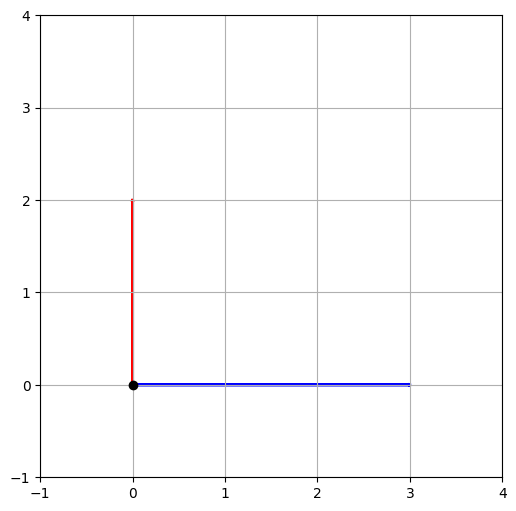
\includegraphics[scale=0.4]{images/vector_addition0.png}}
    \only<2>{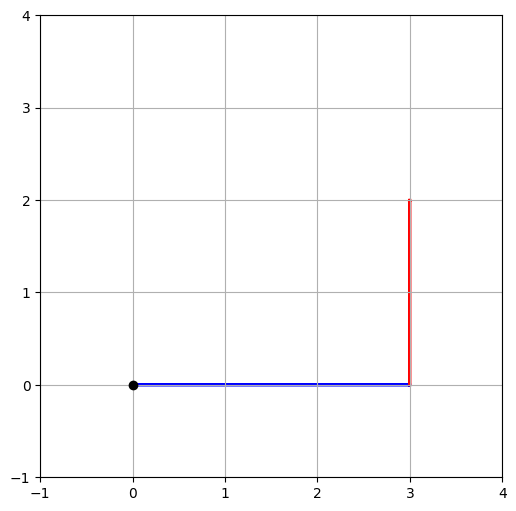
\includegraphics[scale=0.4]{images/vector_addition1.png}}
    \only<3>{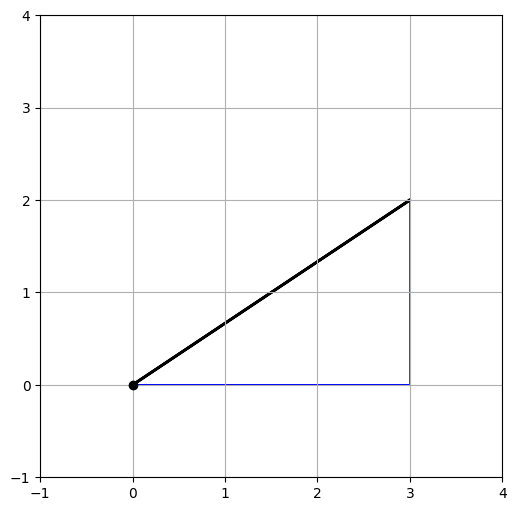
\includegraphics[scale=0.4]{images/vector_addition2.png}}
    \end{columns}
\end{frame}
\againframe<2-3>{vadd}
\againframe{vectors}

\begin{frame}<1>[label=vscale]{Vector Scaling}
    We can scale this vector too.
    \begin{columns}
    \column{0.4\textwidth}
    \centering
    \begin{math}
        \frac{1}{2} * \begin{pmatrix}
            3 \\ 2
        \end{pmatrix}
        = \begin{pmatrix}
            1.5 \\ 1
        \end{pmatrix}
    \end{math}
    \column{0.6\textwidth}
    \only<1>{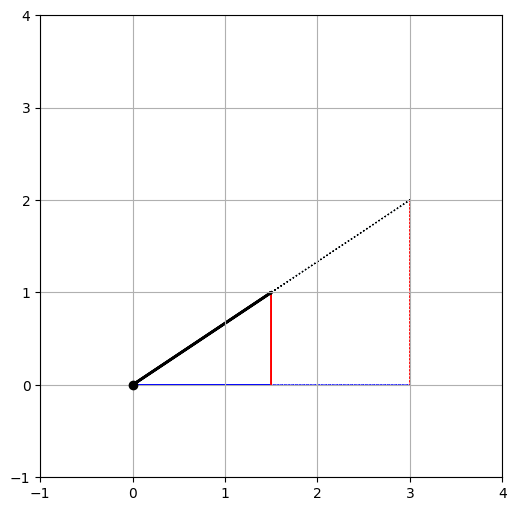
\includegraphics[scale=0.4]{images/vector_scaling.png}}
    \end{columns}
\end{frame}
\againframe{vectors}
\againframe<2>{statevec}

\begin{frame}{Vector Product}
    The inner product we've been using looks very neat with vectors.

    \begin{center}
        \begin{math}
            \braket{0}{0} = 
            \begin{pmatrix}
                1 & 0
            \end{pmatrix}
            \begin{pmatrix}
                1 \\ 0
            \end{pmatrix}
            = 1*1 + 0*0 = 1
        \end{math}
    \end{center}
    Generally, 
    \begin{center}
        \begin{math}
            \braket{x}{y}=
            \begin{pmatrix}
                \textcolor{red}{a} & \textcolor{blue}{b}
            \end{pmatrix}
            \begin{pmatrix}
                \textcolor{red}{c} \\ \textcolor{blue}{d}
            \end{pmatrix}
            =  \textcolor{red}{ac} + \textcolor{blue}{bd}
        \end{math}
    \end{center}
\end{frame}

\begin{frame}<1>[label=vecprod]{Inner Product}
    We can think of the inner product graphically too.\\
    \begin{center}
        \begin{math}
            \braket{x}{y}=
            \begin{pmatrix}
                \textcolor{red}{3} & \textcolor{red}{0}
            \end{pmatrix}
            \begin{pmatrix}
                \textcolor{blue}{2} \\ \textcolor{blue}{2}
            \end{pmatrix}
        \end{math}\\
    \end{center}
    \begin{columns}
        \column{0.5\textwidth}
        \centering
        \only<2->{First we project vector \textcolor{red}{x} onto \textcolor{blue}{y}.}\vfill
        \only<2->{Then we find the length of the new projected vector $\abs{z}$.}\vfill
        \only<3->{Finally, we multiply this by the length of $\textcolor{blue}{y}$, $\abs{\textcolor{blue}{y}}$.\\
        $\braket{\textcolor{red}{x}}{\textcolor{blue}{y}} = \abs{z}\abs{\textcolor{blue}{y}}$}
        \column{0.5\textwidth}
        \only<1>{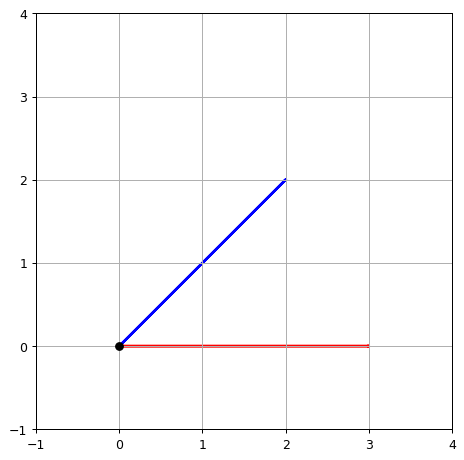
\includegraphics[width=0.8\textwidth]{images/fig1.png}}
        \only<2>{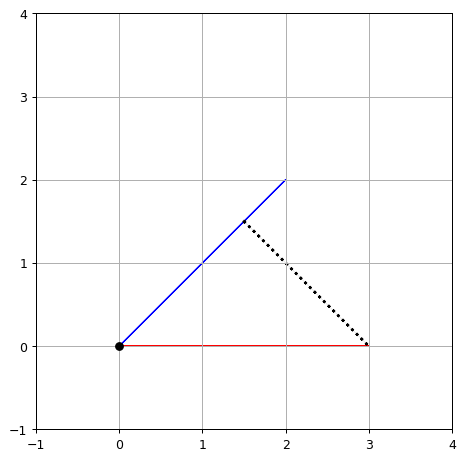
\includegraphics[width=0.8\textwidth]{images/fig2.png}}
        \only<3>{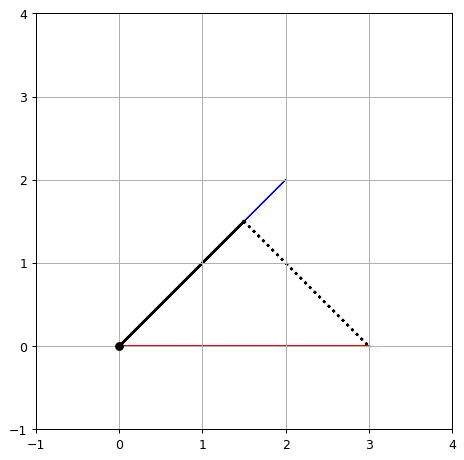
\includegraphics[width=0.8\textwidth]{images/fig3.png}}
    \end{columns}
    
\end{frame}
\againframe<2>{vecprod}
\againframe<3>{vecprod}

\begin{frame}{Orthogonal States}
    By using this projection method, we see that two orthogonal (perpendicular) states have an inner product of 0.
    \begin{columns}
        \column{0.5\textwidth}
        \centering
        \begin{math}
            \braket{x}{y}=
            \begin{pmatrix}
                3 & 0
            \end{pmatrix}
            \begin{pmatrix}
                0 \\ 2
            \end{pmatrix} = 0
        \end{math}
        \column{0.5\textwidth}
        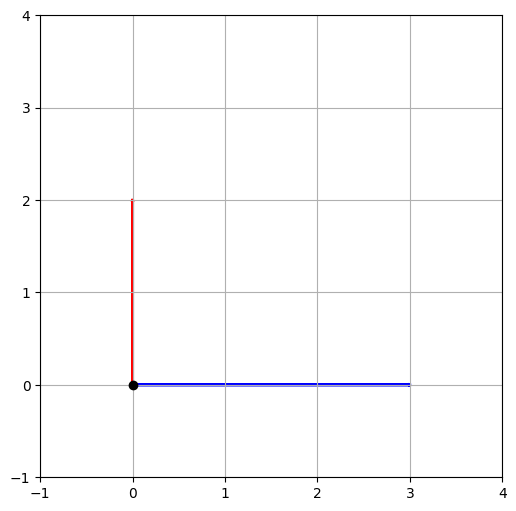
\includegraphics[width=\columnwidth]{images/vector_addition0.png}
    \end{columns}
    
\end{frame}

\begin{frame}{Computational Basis}
    Writing our two states $\ket{0}$ and $\ket{1}$ in this way allows us to make any 2 dimensional vector from a combination of them.\vfill
    \centering
    \begin{columns}
        \column{0.5\textwidth}
        \centering
        \begin{math}
            \ket{0} = \begin{pmatrix}
                1 \\ 0
            \end{pmatrix}
        \end{math}
        \column{0.4\textwidth}
        \centering
        \begin{math}
            \ket{1} = \begin{pmatrix}
                0 \\ 1
            \end{pmatrix}
        \end{math}
    \end{columns}\vfill
    \begin{center}
        \begin{math}
            \begin{pmatrix}
                a \\ b
            \end{pmatrix}
            = a \begin{pmatrix}
                1 \\ 0
            \end{pmatrix}
            + b \begin{pmatrix}
                0 \\ 1
            \end{pmatrix}
        \end{math}\vfill
    \end{center}
    We can this property \textbf{spanning} the 2d vectors.
\end{frame}

\begin{frame}{Computational Basis}
    Additionally, they cannot be written as linear combinations of each other.
    \begin{center}
        \begin{math}
            a\begin{pmatrix}
                1 \\ 0
            \end{pmatrix}
            \ne b \begin{pmatrix}
                0 \\ 1
            \end{pmatrix}
        \end{math}
    \end{center}
    \pause
    They are therefore \textbf{linearly independent}.\vfill
    Spanning and linear independence are the two criteria that make a set of vectors a basis.\vfill
    \pause
    $\{\ket{0}, \ket{1}\}$ is called the \textbf{computational basis} because it relates most clearly to states of bits.\\
\end{frame}
    
\begin{frame}{X Basis}s
    Spanning and linear independence seem pretty obvious for the computational basis, but we could make a basis from a different set of vectors.\vfill
    \begin{columns}
        \column{0.5\textwidth}
        \centering
        \begin{math}
            \ket{+} = \frac{1}{\sqrt{2}}\begin{pmatrix}
                1 \\ 1
            \end{pmatrix}
        \end{math}
        \column{0.4\textwidth}
        \centering
        \begin{math}
            \ket{-} = \frac{1}{\sqrt{2}}\begin{pmatrix}
                1 \\ -1
            \end{pmatrix}
        \end{math}
    \end{columns}\vfill
    \pause
    \begin{columns}
        \column{0.5\textwidth}
        \centering
        \begin{math}
            \ket{+} = \frac{1}{\sqrt{2}}\ket{0} + \frac{1}{\sqrt{2}}\ket{1}
        \end{math}
        \column{0.4\textwidth}
        \centering
        \begin{math}
            \ket{-} = \frac{1}{\sqrt{2}}\ket{0} - \frac{1}{\sqrt{2}}\ket{1}
        \end{math}
    \end{columns}\vfill
    \pause
    The basis $\{\ket{+}, \ket{-}\}$ is called the X basis, for reasons we'll see soon.\vfill
    \pause
    \begin{block}{Exercise}
        Show that the set $\{\ket{+}, \ket{-}\}$ is a basis for the 2d vectors.
    \end{block}
\end{frame}

\begin{frame}{Multi-bit States}
To combine single bit states into larger sizes we use a \emph{tensor product}.\vfill

\centering
\begin{math}
    \ket{x} \otimes \ket{y}
    = \ket{xy}
\end{math}\vfill
\begin{math}
    \begin{pmatrix}
        a_0 \\ b_0
    \end{pmatrix}
    \otimes
    \begin{pmatrix}
        \textcolor{red}{a_1} \\ \textcolor{blue}{b_1}
    \end{pmatrix}
    = 
    \begin{pmatrix}
        a_0
        \begin{pmatrix}
            \textcolor{red}{a_1} \\ \textcolor{blue}{b_1}
        \end{pmatrix}
    \\ b_0
        \begin{pmatrix}
            \textcolor{red}{a_1} \\ \textcolor{blue}{b_1}
        \end{pmatrix}
    \end{pmatrix}
    =
    \begin{pmatrix}
        a_0 \textcolor{red}{a_1} \\ a_0 \textcolor{blue}{b_1} \\ b_0 \textcolor{red}{a_1} \\ b_0 \textcolor{blue}{b_1}
    \end{pmatrix}
\end{math}
\end{frame}

\begin{frame}{Matrices}
    A \textbf{Matrix} can be thought of as a collection of vectors.
    \begin{center}
        \begin{math}
            M =
            \begin{pmatrix}
                a_0 & b_0 & c_0 \\
                a_1 & b_1 & c_1 \\
                a_2 & b_2 & c_2 \\
            \end{pmatrix}
        \end{math}
    \end{center}
\end{frame}

\begin{frame}{Rules for Matrices}
    Matrices behave quite similarly to vectors.\vfill
    With two matrices $\hat{X} = \begin{pmatrix}a_0 & b_0 \\ c_0 & d_0 \end{pmatrix} $ and $\hat{Y} = \begin{pmatrix}a_1 & b_1 \\ c_1 & d_1 \end{pmatrix} $\vfill

    \centering
    \begin{tabular}{c | c}
        \textbf{Addition} & \textbf{Scalar Multiplication}\\[2ex]
        \begin{math}
            \hat{X}+\hat{Y} = \begin{pmatrix}
                a_0+a_1 & b_0+b_1 \\
                c_0 + c_1 & d_0+d_1
            \end{pmatrix}
        \end{math} & \begin{math}
            n * \hat{X} = \begin{pmatrix}
                n * a_0 & n * b_0 \\
                n * c_0 & n * d_0 
            \end{pmatrix}
        \end{math}\\
    \end{tabular}
    
\end{frame}

\begin{frame}{Matrix Multiplication}
When a matrix multiplies a vector, it transforms the vector to a new one.\vfill
    \begin{center}
        
    \begin{math}
        \hat{X}\ket{y} = \begin{pmatrix}
            \color{red} a_0 & \color{red} b_0 \\ \color{blue} c_0 & \color{blue} d_0
            \end{pmatrix} 
            \begin{pmatrix}
                \alpha \\ \beta    
            \end{pmatrix}
            =
            \begin{pmatrix}
                \color{red} a_0 \color{black}\alpha + \color{red} b_0 \color{black}\color{black}\color{black}\beta \\
                \color{blue} c_0 \color{black}\color{black}\alpha + \color{blue} d_0 \color{black}\beta \\       
            \end{pmatrix}
    \end{math}
    \end{center}
    \vfill
    This just gives us another vector.
    \begin{block}{Exercise}
        Find the vector $\nu$:\vfill
        \centering
        \begin{math}
        \nu=
            \begin{pmatrix}
                2 & 7 \\ -2 & 1
            \end{pmatrix}
            \begin{pmatrix}
                -4 \\ 3
            \end{pmatrix}
        \end{math}
    \end{block}
\end{frame}

\begin{frame}{Matrix Multiplication}
Similarly matrices can be multiplied together\vfill
    \centering
    \begin{math}
        \hat{X}\hat{Y} = \begin{pmatrix}
            \color{red} a_0 & \color{red} b_0 \\ \color{blue} c_0 & \color{blue} d_0
            \end{pmatrix} 
            \begin{pmatrix}
                \alpha & \color{orange}\gamma \\ \beta & \color{orange}\delta    
            \end{pmatrix}
            =
            \begin{pmatrix}
                \color{red} a_0 \color{black}\alpha + \color{red} b_0 \color{black}\color{black}\color{black}\beta &
                \color{red} a_0 \color{orange}{\gamma} \color{black}+ \color{red} b_0 \color{black}\color{black}\color{orange}\delta
                \\
                \color{blue} c_0 \color{black}\color{black}\alpha + \color{blue} d_0 \color{black}\beta &
                \color{blue} c_0 \color{black}\color{orange}{\gamma}\color{black} + \color{blue} d_0 \color{orange}\delta\\       
            \end{pmatrix}
    \end{math}\vfill
    \pause
    \begin{block}{Exercise}
        Find the matrix $M$:\vfill
        \centering
        \begin{math}
        M=
            \begin{pmatrix}
                2 & 7 \\ -2 & 1
            \end{pmatrix}
            \begin{pmatrix}
                -4 & 0 \\ 3 & 3
            \end{pmatrix}
        \end{math}
    \end{block}
\end{frame}
% \begin{frame}{Matrix Multiplication}
%     We can now see how to relate our two kinds of notation!\vfill
%     \centering
%     \begin{math}
%         \hat{N}\ket{0} = \ket{1}
%     \end{math}\vfill
%     \begin{math}
%         \begin{pmatrix}
%             0 & 1 \\ 1 & 0
%         \end{pmatrix}
%         \begin{pmatrix}
%             1 \\ 0
%         \end{pmatrix}
%         = \begin{pmatrix}
%             0*1 + 1*0 \\ 1*1 + 0*0
%         \end{pmatrix}
%         = 
%         \begin{pmatrix}
%             0 \\ 1
%         \end{pmatrix}
%     \end{math}\vfill
%     \begin{math}
%         \hat{N} = \begin{pmatrix}
%             0 & 1 \\ 1 & 0
%         \end{pmatrix}
%     \end{math}
% \end{frame}


\begin{frame}{Matrix Form of Operators}
    \begin{columns}
        \column{0.5\textwidth}
        \centering
        \begin{math}
            \hat{N}\ket{0}
        \end{math}\vfill
        \column{0.5\textwidth}
        \centering
        \begin{math}
            \hat{N}\ket{1}
        \end{math}
    \end{columns}\vfill
    \pause
    \begin{columns}
        \column{0.5\textwidth}
        \centering
        \begin{math}
            \hat{N}
            \begin{pmatrix}
                1 \\ 0
            \end{pmatrix}
        \end{math}
        \column{0.5\textwidth}
        \centering
        \begin{math}
            \hat{N}
            \begin{pmatrix}
                0 \\ 1
            \end{pmatrix}
        \end{math}
    \end{columns}\vfill
    \pause
    \begin{columns}
        \column{0.5\textwidth}
        \centering
        \begin{math}
            \begin{pmatrix}
                0 & 1 \\ 1 & 0
            \end{pmatrix}
            \begin{pmatrix}
                1 \\ 0
            \end{pmatrix}
        \end{math}
        \column{0.5\textwidth}
        \centering
        \begin{math}
            \begin{pmatrix}
                0 & 1 \\ 1 & 0
            \end{pmatrix}
            \begin{pmatrix}
                0 \\ 1
            \end{pmatrix}
        \end{math}
    \end{columns}\vfill
    \pause
    \begin{columns}
        \column{0.5\textwidth}
        \centering
        \begin{math}
            \begin{pmatrix}
                0 & 1 \\ 1 & 0
            \end{pmatrix}
            \begin{pmatrix}
                1 \\ 0
            \end{pmatrix}
            = 
            \begin{pmatrix}
                0 \\ 1
            \end{pmatrix}
        \end{math}
        \column{0.5\textwidth}
        \centering
        \begin{math}
            \begin{pmatrix}
                0 & 1 \\ 1 & 0
            \end{pmatrix}
            \begin{pmatrix}
                0 \\ 1
            \end{pmatrix}
            = 
            \begin{pmatrix}
                1 \\ 0
            \end{pmatrix}
        \end{math}
    \end{columns}\vfill
\end{frame}

\begin{frame}{Matrix form of Operators}
    We can actually find out the matrix form of an operator from its outer product form.\vfill
    \centering
    \begin{math}
        \hat{N} = \ket{1}\bra{0} + \ket{0}\bra{1}
    \end{math}\vfill
    \pause
    \begin{math}
        \hat{N} = \textcolor{red}{0}\ket{0}\bra{0} + \textcolor{red}{1}\ket{1}\bra{0} + \textcolor{red}{1}\ket{0}\bra{1} + \textcolor{red}{0}\ket{1}\bra{1}
    \end{math}
    \vfill
    \pause
    $\hat{N} = $\begin{tabular}{c c}
            $\textcolor{red}{0}\ket{0}\bra{0}$ & $\textcolor{red}{1}\ket{0}\bra{1}$\\
            $\textcolor{red}{1}\ket{1}\bra{0}$ & $\textcolor{red}{0}\ket{1}\bra{1}$
    \end{tabular}
    \vfill
    \pause
    \begin{math}
        \hat{N} = 
        \begin{pmatrix}
            0 & 1 \\ 1 & 0
        \end{pmatrix}
    \end{math}
\end{frame}

\begin{frame}{Multi-bit Operators}
    The \textbf{only} time an AND gate returns $ON$ is when we have both inputs on.\vfill

    \begin{center}
    \begin{math}
        \hat{A}\ket{11} = \ket{1}
    \end{math}\vfill
    \begin{math}
        \centering
        \ket{11}=
        \begin{pmatrix} 0 \\ 1 \end{pmatrix} 
        \otimes 
        \begin{pmatrix} 0 \\ 1 \end{pmatrix} 
        =
        \begin{pmatrix} 0 \\ 0 \\ 0 \\ 1 \end{pmatrix} 
    \end{math}

    \begin{math}
        \hat{A}\begin{pmatrix} 0 \\ 0 \\ 0 \\ 1 \end{pmatrix} = \begin{pmatrix} 0 \\ 1 \end{pmatrix} 
    \end{math}
    \end{center}
\end{frame}

\begin{frame}{Multi-bit Operators}
    The $\hat{A}$ operator has the form:\vfill
    \centering
    \begin{math}
        \hat{A} = \begin{pmatrix}
            1 & 1 & 1 & 0 \\
            0 & 0 & 0 & 1
        \end{pmatrix}
    \end{math}\vfill
    \begin{math}
        \begin{pmatrix}
            1 & 1 & 1 & 0 \\
            0 & 0 & 0 & 1
        \end{pmatrix}
        \begin{pmatrix} 0 \\ 0 \\ 0 \\ 1 \end{pmatrix} = \begin{pmatrix} 0 \\ 1 \end{pmatrix} 
    \end{math}
\end{frame}
 
\begin{frame}{Multi-bit Operators}
    and the \textbf{only} time an OR gate returns $OFF$ is when we have both inputs off.
    \vfill

    \begin{center}
    \begin{math}
        \hat{O}\ket{00} = \ket{0}
    \end{math}\vfill
    \begin{math}
        \ket{00} =
        \begin{pmatrix} 1 \\ 0 \end{pmatrix} 
        \otimes 
        \begin{pmatrix} 1 \\ 0 \end{pmatrix} 
        =
        \begin{pmatrix} 1 \\ 0 \\ 0 \\ 0 \end{pmatrix} 
    \end{math}

    \begin{math}
        \hat{O}\begin{pmatrix} 1 \\ 0 \\ 0 \\ 0 \end{pmatrix} = \begin{pmatrix} 1 \\ 0 \end{pmatrix}
    \end{math}
    \end{center}
\end{frame}

\begin{frame}{Multi-bit Operators}
    The $\hat{0}$ operator has the form:\vfill
    \centering
    \begin{math}
        \hat{0} = \begin{pmatrix}
            1 & 0 & 0 & 0 \\
            0 & 1 & 1 & 1 
        \end{pmatrix}
    \end{math}\vfill
    \begin{math}
        \begin{pmatrix}
            1 & 0 & 0 & 0 \\ 
            0 & 1 & 1 & 1 
        \end{pmatrix}
        \begin{pmatrix} 1 \\ 0 \\ 0 \\ 0 \end{pmatrix} = \begin{pmatrix} 1 \\ 0 \end{pmatrix} 
    \end{math}
\end{frame}

\begin{frame}{Logic Summary}
    We now have three(!) equivalent ways of thinking about computational logic.\vfill
    \begin{enumerate}
        \item Circuits
        \item States and Operators
        \item Vectors and Matrices
    \end{enumerate}\vfill
    These are the same tools we'll use to understand quantum algorithms later on.
\end{frame}




%%%%%%%%%%%%%%%%%%%%%%%%%%%%%%%%%%%%%%%%%%%%%%%%%%%%%%%
\section{Quantum Circuits}
\begin{frame}{Components}
\begin{itemize} 
    \item Quantum circuits flow from left to right.\\
    \pause
    \item We use a wire to represent each qubit.\\
    \item Wires cannot be split. (No FANOUT)\\
    \pause
    \item Boxes represent Operators.\\
    \pause
    \item Each qubit starts in state $\ket{0}$ unless stated otherwise.\\
    \pause
\end{itemize}
\vfill
\centering
\begin{quantikz}
    \lstick{$q_0$} & \phantomgate{1} &\phantomgate{1} &\gate{U}&\phantomgate{1} & \phantomgate{1}\\
    \lstick{$q_1$} & \phantomgate{1} &\phantomgate{1} &\phantomgate{1}&\phantomgate{1} & \phantomgate{1}\\
\end{quantikz}
\end{frame}


\begin{frame}{Pauli Matrices}
    \begin{columns}
        \column{0.3\textwidth}
        \centering
        \begin{math}
        \sigma_{X} =
            \begin{pmatrix}
                0 & 1 \\ 1 & 0
            \end{pmatrix}
        \end{math}
        \column{0.3\textwidth}
        \centering
        \begin{math}
        \sigma_{Y} =
            \begin{pmatrix}
                0 & -i \\ i & 0
            \end{pmatrix}
        \end{math}
        \column{0.3\textwidth}
        \centering
        \begin{math}
        \sigma_{Z} =
            \begin{pmatrix}
                1 & 0 \\ 0 & -1
            \end{pmatrix}
        \end{math} 
    \end{columns}
    \vfill    
\end{frame}

\begin{frame}{Pauli Matrices}
    Once we add in the identity $\mathbb{I}= \begin{pmatrix} 1 & 0 \\ 0 & 1 \end{pmatrix}$, we have a \textbf{basis} for the $2x2$ matrices.\vfill
    \begin{block}{Exercise}
        Show that the set $\{\sigma_x,\sigma_y,\sigma_z, I\}$ is a basis for the $2x2$ matrices.
    \end{block}
%\centering
%     \begin{math}
%         M = \alpha\sigma_x + \beta\sigma_y + \gamma\sigma_z + \delta \mathbb{I}
%     \end{math}
\end{frame}

\begin{frame}{Pauli Matrices}
    Prove that the Pauli matrices are self-inverse.
\vfill
\centering
    \begin{columns}
        \column{0.3\textwidth}
        \centering
        \begin{math}
        \sigma_{X} =
            \begin{pmatrix}
                0 & 1 \\ 1 & 0
            \end{pmatrix}
        \end{math}
        \column{0.3\textwidth}
        \centering
        \begin{math}
        \sigma_{Y} =
            \begin{pmatrix}
                0 & -i \\ i & 0
            \end{pmatrix}
        \end{math}
        \column{0.3\textwidth}
        \centering
        \begin{math}
        \sigma_{Z} =
            \begin{pmatrix}
                1 & 0 \\ 0 & -1
            \end{pmatrix}
        \end{math} 
    \end{columns}\vfill
    \begin{math}
        \sigma_{X}\sigma_{X} = \sigma_{Y}\sigma_{Y} = \sigma_{Z}\sigma_{Z} = \mathbb{I}
    \end{math}
\end{frame}

\begin{frame}{Pauli Gates}
    \begin{columns}
        \column{0.3\textwidth}
        \centering
        \begin{math}
        \sigma_{X} =
            \begin{pmatrix}
                0 & 1 \\ 1 & 0
            \end{pmatrix}
        \end{math}
        \column{0.3\textwidth}
        \centering
        \begin{math}
        \sigma_{Y} =
            \begin{pmatrix}
                0 & -i \\ i & 0
            \end{pmatrix}
        \end{math}
        \column{0.3\textwidth}
        \centering
        \begin{math}
        \sigma_{Z} =
            \begin{pmatrix}
                1 & 0 \\ 0 & -1
            \end{pmatrix}
        \end{math} 
    \end{columns}
    \vfill    
   \begin{columns}
        \column{0.3\textwidth}
        \centering
        \begin{quantikz}
            \phantomgate{1} & \gate{X} & \phantomgate{1}
        \end{quantikz}
        \column{0.3\textwidth}
        \centering
        \begin{quantikz}
            \phantomgate{1} & \gate{Y} & \phantomgate{1}
        \end{quantikz}
        \column{0.3\textwidth}
        \centering
        \begin{quantikz}
            \phantomgate{1} & \gate{Z} & \phantomgate{1}
        \end{quantikz}
        \end{columns}
\end{frame}

\begin{frame}{Hadamard Gate}
One of the most common gates is the Hadamard gate, which maximally mixes the $\ket{0}$ and $\ket{1}$ states.\vfill
\centering
\begin{math}
    H = \frac{1}{\sqrt{2}}\begin{pmatrix}
        1 & 1 \\ 1 & -1
    \end{pmatrix}
\end{math}\vfill

so $\hat{H}\ket{0} = (\ket{0} + \ket{1})/\sqrt{2}$ and $\hat{H}\ket{1} = (\ket{0} - \ket{1})/\sqrt{2}$.
\vfill

Which puts the state half way between $\ket{0}$ and $\ket{1}$.
\end{frame}

\begin{frame}{Visualising Gates}
    Let's visualise the action of these one qubits gates using the Bloch Sphere.
    \note{If gifs don't work then pull them up here.}
    \begin{center}
        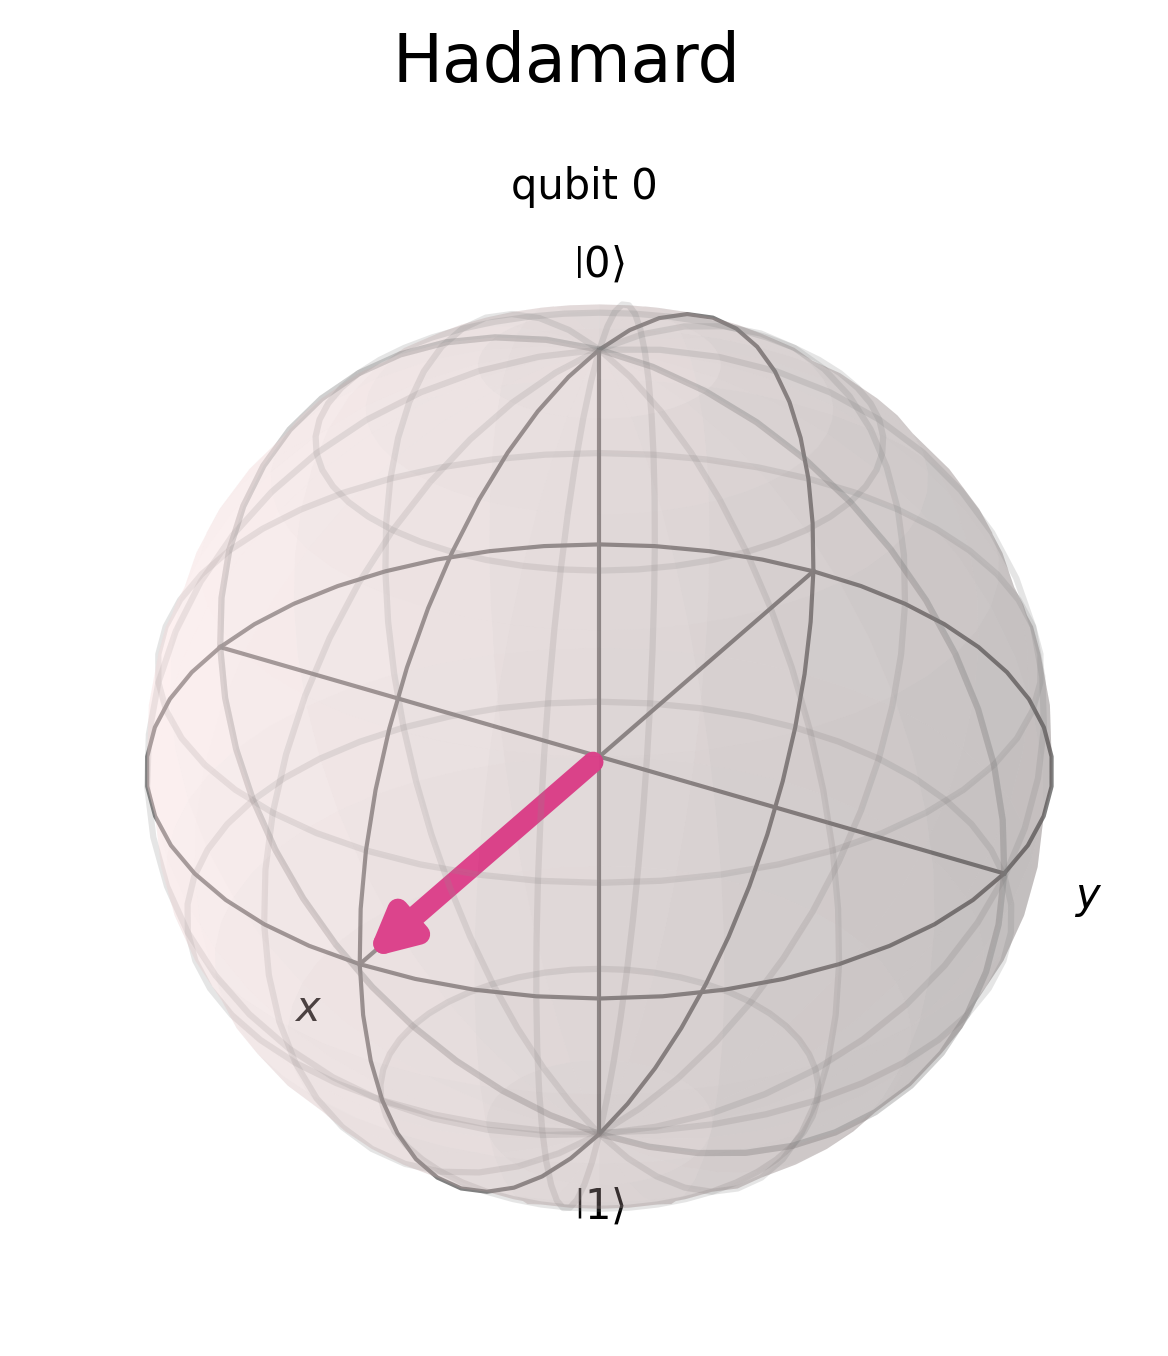
\includegraphics[width=0.4\textwidth]{images/bloch_H.png}
    \end{center}
    \movie[]{}{images/Bloch_R_X.gif}
    \vfill
    We can see that the Hadamard gate has moved the state so that it now points along the x-axis of the bloch sphere.\vfill
    This is the $\ket{+}$ state, with the $\ket{-}$ being at the opposite side of the sphere.
    
\end{frame}

\begin{frame}{Visualising Gates}
    We know that for a state $\ket{\Psi} = \alpha\ket{0} + \beta\ket{1}$ we expect:\vfill
    \begin{center}
        \begin{math}
            \hat{X}\ket{\Psi} = \alpha\ket{1} + \beta\ket{0}
        \end{math}
    \end{center}\vfill
    Lets visualise this on the bloch sphere:\vfill
    \begin{columns}
        \column{0.5\textwidth}
        
    \end{columns}
    
\end{frame}

\begin{frame}{Rotation Gates}
    We can turn these into rotations by an angle $\theta$ by mixing them with the identity.\vfill
    \centering
    \begin{math}
        R_X =\cos{\frac{\theta}{2}}\mathbb{I} - i \sin{\frac{\theta}{2}}\sigma_x
    \end{math}\vfill

    \centering
    \begin{math}
    R_{X} =
        \begin{pmatrix}
            \cos{\frac{\theta}{2}} & -i\sin{\frac{\theta}{2}} \\ -i\sin{\frac{\theta}{2}} & \cos{\frac{\theta}{2}}
        \end{pmatrix}
    \end{math}\vfill
    \centering
    \begin{quantikz}
        \phantomgate{1} & \gate{R_X} & \phantomgate{1}
    \end{quantikz}
\end{frame}

\begin{frame}{Rotation Gates}
    \centering
    \begin{math}
        R_Y = \cos{\frac{\theta}{2}}\mathbb{I} - i \sin{\frac{\theta}{2}}\sigma_y
    \end{math}\vfill
        \centering
        \begin{math}
        R_{Y} =
            \begin{pmatrix}
                \cos{\frac{\theta}{2}} & -\sin{\frac{\theta}{2}} \\ \sin{\frac{\theta}{2}} & \cos{\frac{\theta}{2}}
            \end{pmatrix}
        \end{math}\vfill
        \begin{quantikz}
            \phantomgate{1} & \gate{R_Y} & \phantomgate{1}
        \end{quantikz}
\end{frame}

\begin{frame}{Rotation Gates}
    \centering
    \begin{math}
        R_Z = \cos{\frac{\theta}{2}}\mathbb{I} - i \sin{\frac{\theta}{2}}\sigma_z
    \end{math}\vfill
        \centering
        \begin{math}
        R_{Z} =
            \begin{pmatrix}
                \cos{\frac{\theta}{2}} -  i\sin{\frac{\theta}{2}} & 0 \\ 0 & \cos{\frac{\theta}{2}} + i\sin{\frac{\theta}{2}}
            \end{pmatrix}
        \end{math}\vfill
        \begin{quantikz}
            \phantomgate{1} & \gate{R_Z} & \phantomgate{1}
        \end{quantikz}
\end{frame}

\begin{frame}{Two-qubit Gates}
\centering
Controlled-NOT
\vfill
\begin{quantikz}
    \phantomgate{1} & \ctrl{1} & \phantomgate{1} & \\
    \phantomgate{1} & \targ{} & \phantomgate{1} &
\end{quantikz}
\vfill
\begin{math}
    U_{CN} =
    \begin{pmatrix}
        1 & 0 & 0 & 0 \\
        0 & 1 & 0 & 0 \\
        0 & 0 & 0 & 1 \\
        0 & 0 & 1 & 0
    \end{pmatrix}
\end{math}
\end{frame}

\begin{frame}{Swap Gate}
We can swap the states of two qubits using three CNOT gates.
\vfill
\centering
    \begin{quantikz}
        \phantomgate{1} & \ctrl{1} & \targ{} & \ctrl{1} & \phantomgate{1} & \\
        \phantomgate{1} & \targ{} & \ctrl{-1} & \targ{} & \phantomgate{1} &
    \end{quantikz}
    =
    \begin{quantikz}
        \phantomgate{1} & \swap{1} & \phantomgate{1} \\
        \phantomgate{1} & \targX{} & \phantomgate{1}
    \end{quantikz}
\vfill
\end{frame}

\begin{frame}{Measurement}
    The last basic component is the measurement symbol, which will terminate the line.
    \vfill
    \centering
    \begin{quantikz}
       \lstick{$\ket{0}$} & \gate{H} & \ctrl{1} & \phantomgate{1}\\
        \lstick{$\ket{0}$} & \phantomgate{1} & \targ{} & \meter{}
    \end{quantikz}
\end{frame}

\begin{frame}{IMBQ}
    Now we're ready to run our first quantum circuits.\\
    We're going to do this using a Jupyter notebook 
    % We're going to use \href{https://quantum-computing.ibm.com/composer}{IMB Quantum Composer} to do this.\\
    % If you haven't got one already you'll need to.
\end{frame}

\begin{frame}{Metrics}
    The size of circuits is measured with two different numbers.

    \begin{enumerate}
        \item Depth - The maximum number of gates which have to be applied in sequence.
        \item Qubit Count - The maximum number of qubits in use at any one time.
    \end{enumerate}
    
\end{frame}

\begin{frame}{Depth}
    Depth is calculated as the maximum number of gates which must be applied in sequence.
    \vfill
    \centering
    \movie[width=0.3\textwidth]{}{images/depth.gif}
\end{frame}

\begin{frame}{Qubit Count}
    Qubit count is the maximum number of physical qubits that have to be in use at any one time.\\
    \begin{center}
    \begin{quantikz}
       \lstick{$\ket{0}$} & \gate{H} & \ctrl{1} & \phantomgate{1} \\
        \lstick{$\ket{0}$} & \phantomgate{1} & \targ{} & \meter{}\\
        \lstick{$\ket{0}$} & \phantomgate{1} & \phantomgate{1} & \phantomgate{1} &
    \end{quantikz}
    \end{center}\vfill
    Even though we have three qubits, the qubit count for this circuit is two.
\end{frame}

%%%%%%%%%%%%%%%%%%%%%%%%%%%%%%%%%%%%%%%%%%%%%%%%%%%%%%%
\section{Information \& Communication}

\begin{frame}[label=info]{Information}
    What sort of things can we do with information?
    \pause
    \begin{itemize}
        \item Read
        \item Edit
        \item Delete
        \item Move
        \item Copy
        \item Encryption / decryption
    \end{itemize}
\end{frame}

\begin{frame}{Readout}
    When we measure a state we get each possible result with some probability.\vfill
    \pause
    We're interested in knowing these probabilities.\vfill
    \pause
    So we have to make lots of measurements.\vfill
    \pause
    Which requires preparing the state each time!
\end{frame}

\againframe{info}

\begin{frame}{No Cloning Theorem}
\begin{theorem}
    There is no operation which can copy arbitrary quantum states.
\end{theorem}\vfill
We prove this by supposing it is possible.\vfill
\begin{columns}
\column{0.5\textwidth}
\centering
\begin{math}
    \ket{\Psi} \otimes \ket{s} \xrightarrow{U} \ket{\Psi} \otimes \ket{\Psi}
\end{math}
\column{0.5\textwidth}
\centering
\begin{math}
    \ket{\Phi} \otimes \ket{s} \xrightarrow{U} \ket{\Phi} \otimes \ket{\Phi}
\end{math}
\end{columns}
\pause
\vfill
\centering
\begin{math}
    (\bra{\Psi} \otimes \bra{s}) (\ket{\Phi} \otimes \ket{s}) = (\bra{\Psi} \otimes \bra{\Psi}) (\ket{\Phi} \otimes \ket{\Phi})
\end{math}\vfill
\pause
\begin{math}
    \braket{\Psi}{\Phi} \otimes \braket{s}{s} = \braket{\Psi}{\Phi} \otimes \braket{\Psi}{\Phi}
\end{math}\vfill
\pause
\begin{math}
    \braket{\Psi}{\Phi} = (\braket{\Psi}{\Phi})^2
\end{math}\vfill
So either $\ket{\Psi}$ and $\ket{\Phi}$ are the same state or they're orthogonal!
\end{frame}

\againframe{info}

\begin{frame}{Private Key Distribution}
    Alice and Bob know they will soon have a message to send over the internet, but it's critical it stays private from their friend Eve.\footnote{They are planning surprise a party for Eve's cat, who is alive and well.}\vfill
    \pause
    They could met up in person ahead of time, and agree on a secret \textbf{key}, a string of random bits.\vfill
    \begin{center}
        \begin{math}
            k = \textcolor{red}{00111000101100101}\dots
        \end{math}
    \end{center}\vfill
\end{frame}

\begin{frame}{Private Key Distribution}
    When the time comes, Alice prepares her message in binary, then adds the key to her own bits modulo 2.\vfill
    \begin{center}
        \begin{math}
            01100010100111011
        \end{math}\vfill     
        \begin{math}
            +
        \end{math}\vfill
        \begin{math}
            \textcolor{red}{00111000101100101}
        \end{math}\vfill
        \begin{math}
            \downarrow
        \end{math}\vfill
        \begin{math}
            01011010001011110
        \end{math}\vfill
    \end{center}
    \pause
    Now her message is encrypted. Bob can decode it by doing the same operation.\footnote{in this case addition and subtraction give the same result. Try it out.}\vfill
    Even if Eve intercepted it the message she couldn't know what the original values were without having the key.
\end{frame}

\begin{frame}{Quantum Key Distribution}
    This system works great provided that:\vfill
    \begin{enumerate}
        \item You know you'll need to send the message
        \item You can meet beforehand
        \item No one steals either copy of the key
    \end{enumerate}\vfill
    It would be much better to create a new key at the time of each message.\vfill
    However, if Alice and Bob tried to send each other messages containing the key before the message, Eve could listen in.
\end{frame}

\begin{frame}{Quantum Key Distribution}
    There is a way that Alice and Bob can create a key for themselves by sending Qubits to each other.\vfill
    \begin{enumerate}
        \item Alice creates two strings of random bits, $a$ and $b$.
        \pause
        \item She encodes the bits of $a$ using the bits of $b$.
        \begin{center}
            \begin{tabular}{|l|c c|}
                \hline
                 & a=0 & a=1 \\
                \hline
                b=0 & $\ket{0}$ & $\ket{1}$ \\
                b=1 & $\ket{+}$ & $\ket{-}$ \\
                \hline
            \end{tabular}
        \end{center}
        
        \pause
        \item She then sends these to Bob.
        \pause
        \item Alice keeps $b$ private for now.
        \pause
        \item Bob picks at random which basis to measure Alice's encoded bits in, and records his choices as $c$.
        \pause
        \item Alice publicly announces $b$.
        \pause
        \item Alice and Bob discard any bits for which $b$ is different from $c$.
    \end{enumerate}
\end{frame}

\begin{frame}{Quantum Key Distribution}
    Let's see an example.
    \begin{center}
        \begin{columns}
            \column{0.5\textwidth}
            \centering
            \begin{math}
                a = \textcolor{blue}{0110011}
            \end{math}\vfill  
            \begin{math}
                b = \textcolor{red}{1011001}
            \end{math}\vfill
            \column{0.5\textwidth}
            \centering
                \begin{tabular}{|l|c c|}
                    \hline
                     & a=0 & a=1 \\
                    \hline
                    b=0 & $\ket{0}$ & $\ket{1}$ \\
                    b=1 & $\ket{+}$ & $\ket{-}$ \\
                    \hline
                \end{tabular}
        \end{columns}
        \begin{math}
            \downarrow
        \end{math}\vfill
        \begin{math}
            \ket{+}\ket{1}\ket{-}\ket{+}\ket{0}\ket{1}\ket{-}
        \end{math}\vfill
        \pause
        \begin{math}
            c = 1110100
        \end{math}\\
        \pause
        \begin{math}
            \downarrow
        \end{math}\vfill
        \begin{math}
            \ket{+}\ket{+}\ket{-}\ket{1}\ket{-}\ket{1}\ket{0}
        \end{math}\\
        \begin{math}
            \downarrow
        \end{math}\vfill
        \pause
        \begin{math}
            0\ \textcolor{red}{0}\ 1\ \textcolor{red}{1}\ \textcolor{red}{0}\ 1\ \textcolor{red}{1}
        \end{math}
    \end{center}
    
\end{frame}

\begin{frame}{Checking for Eavesdropping}
    The No Cloning Theorem prevents Eve from copying the qubits Alice sends to Bob.\vfill
    Lets say she'd like to gain information about which state they share without disturbing the state.\vfill
    \begin{center}
    \begin{math}
        \ket{\psi}\ket{u} \to \ket{\psi}\ket{v}
    \end{math}\\
    \begin{math}
        \ket{\phi}\ket{u} \to \ket{\phi}\ket{v'}
    \end{math}\vfill
    \end{center}    
    \pause

    If Eve can make $\ket{v}$ and $\ket{v'}$ different, then she can tell which state they had!
    \pause
    \begin{center}
    \begin{math}
        \braket{\psi}{\phi}\braket{v}{v'} = \braket{\psi}{\phi}\braket{u}{u}
    \end{math}\vfill
    \begin{math}
        \braket{v}{v'} = \braket{u}{u} = 1
    \end{math}\vfill
    \end{center}
    \pause
Because $\braket{v}{v'} = 1$, they must be the same state. Eve can't learn about Alice and Bob's state without changing it.
\end{frame}

\begin{frame}{Checking for Eavesdropping}
    Alice and Bob can do a final check to see if someone is interfering with their states.\vfill
    \pause
    They remove a portion of their key and share publicly to look for discrepancies.\vfill
    \pause
    If there are too many differences, they know that someone was intercepting the message.\vfill
\end{frame}

%%%%%%%%%%%%%%%%%%%%%%%%%%%%%%%%%%%%%%%%%%%%%%%%%%%%%%%
\section{Hardware}

\begin{frame}{Required properties}
    The criteria for quantum information processing are:
    \begin{itemize}
        \item Well defined two-level system
        \item Ability to initialise the state
        \item Long qubit coherence times\footnote{Compared to the time it takes to implement a gate.}
        \item Universal gate set
        \item Measurement
    \end{itemize}
\end{frame}

\begin{frame}{Desirable properties}
    These are pretty loose criteria but in reality some designs are better than others.
    \begin{itemize}
        \item Low noise
        \item Qubit connectivity
        \item Easy to scale up
        \item Reliable 
        \item Cheap to build and use
    \end{itemize}
\end{frame}

\begin{frame}<0>[label=hardware]{Hardware}
    \note{There are lots of ways to make a quantum computer, although the most common at the moment are:}

    \begin{itemize}
        \item<alert@1> Trapped Ions
        \item<alert@2> Superconducting Qubits
    \end{itemize}
    
\end{frame}

\againframe<1>{hardware}

\begin{frame}{Trapped Ions}
    \begin{figure}
        \centering
        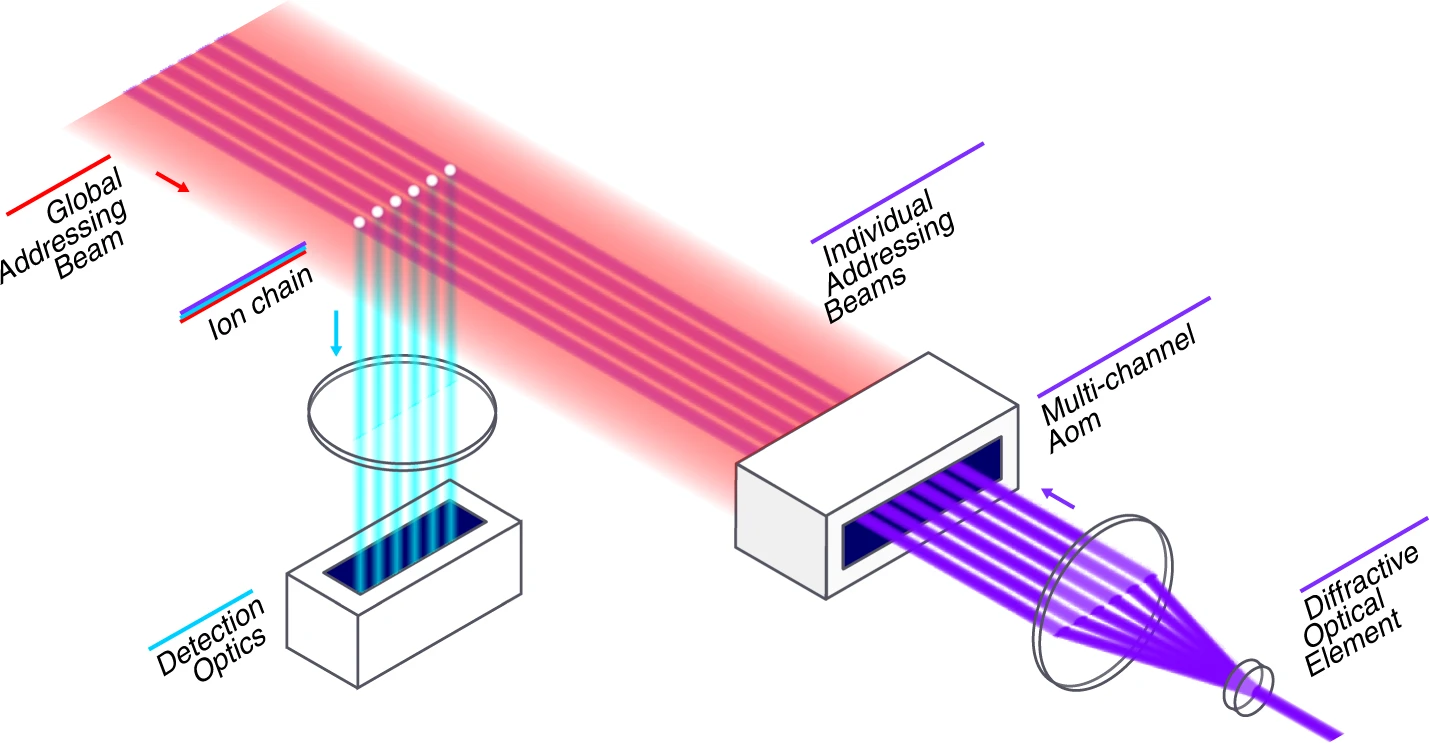
\includegraphics[width=\textwidth]{images/ionq_schematic.png}
        \caption{IONQ}
    \end{figure}
\end{frame}

\begin{frame}{Trapped Ions}
    \begin{figure}
        \centering
        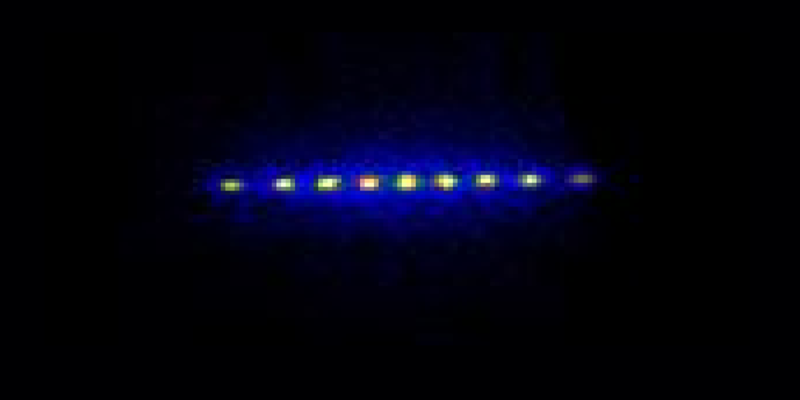
\includegraphics[width=\textwidth]{images/cropion.png}
        \caption{Trapped Ions - University of Oxford}
    \end{figure}
\end{frame}

\begin{frame}{Trapped Ions}
    \begin{figure}
        \centering
        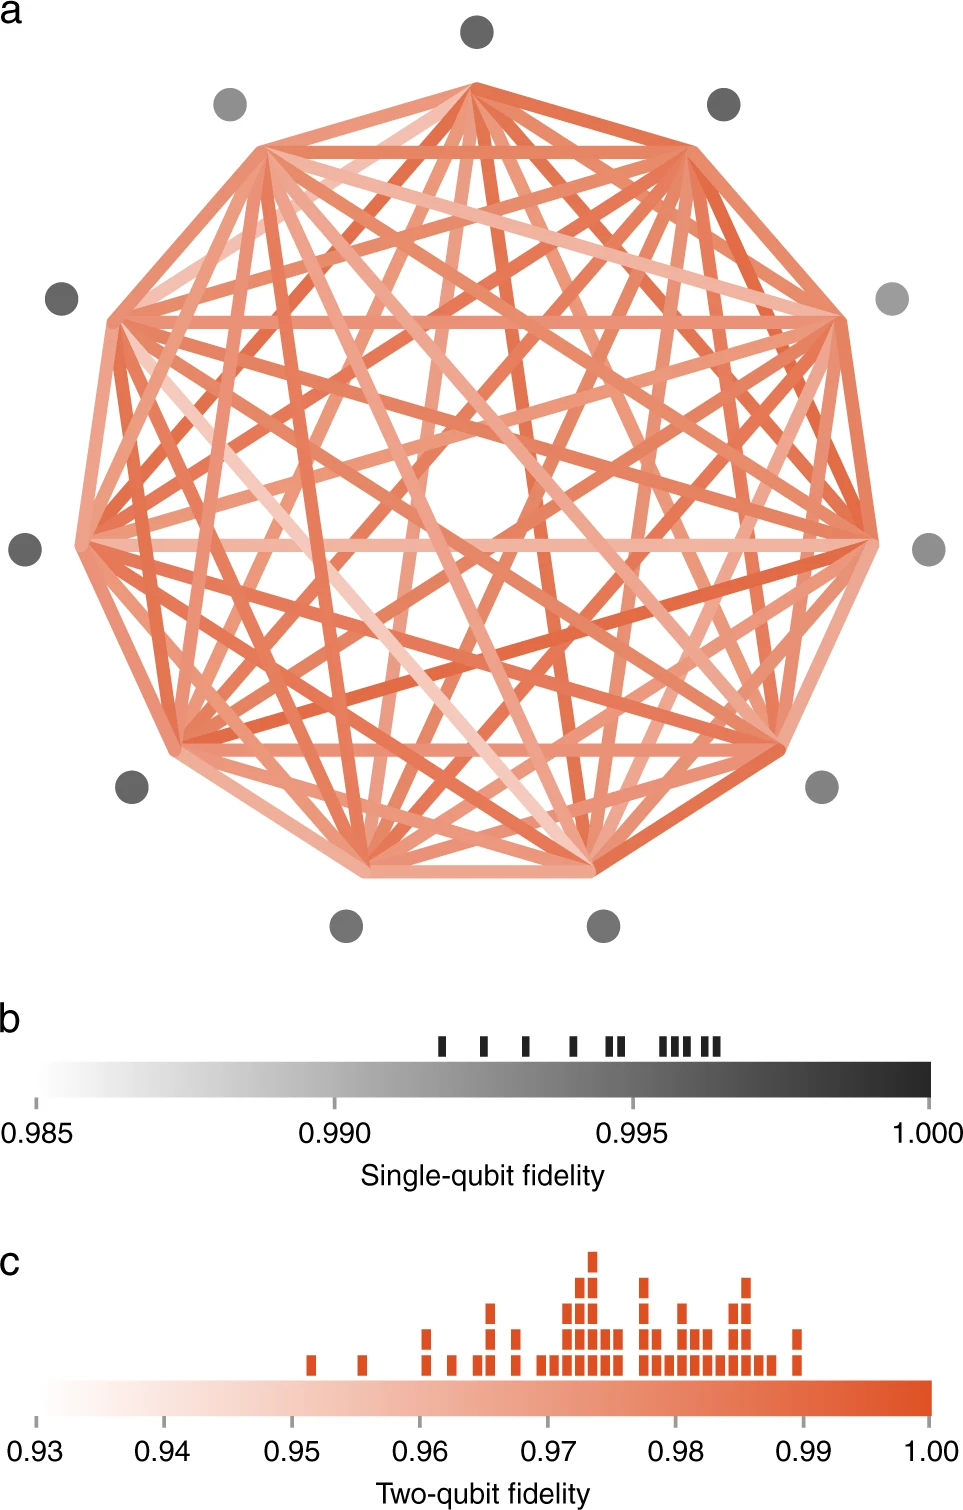
\includegraphics[width=0.4\textwidth]{images/ionq_connectiviy.png}
        \caption{IONQ}
    \end{figure}
\end{frame}

\begin{frame}{Trapped Ions: Connectivity}
    Qubits are defined using two energy levels of the ion.\\
    We can manipulate the energy of the Ion by using a laser with a resonant frequency.\vfill
    \begin{figure}
        \centering
        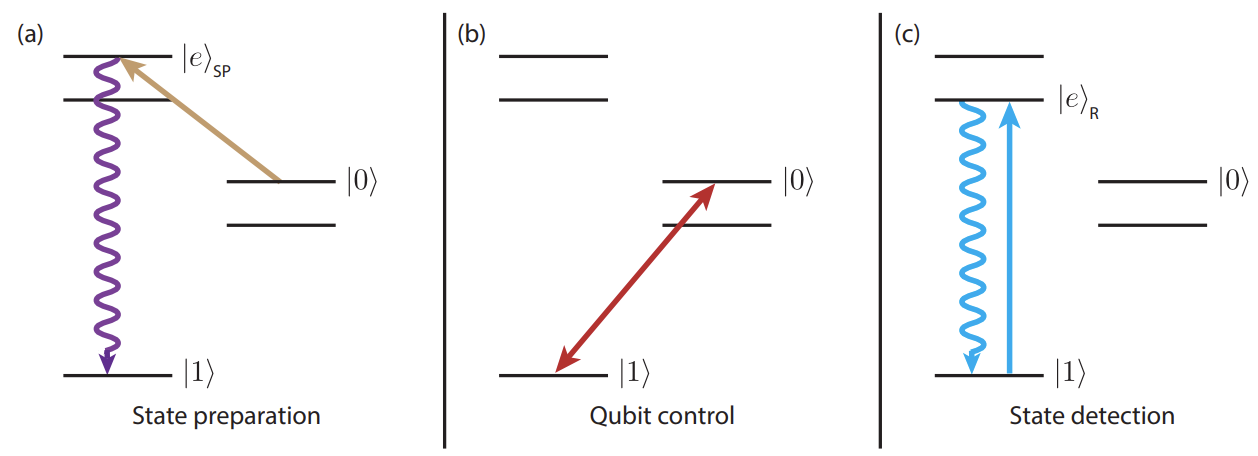
\includegraphics[width=\textwidth]{images/iondiagram.png}
        \caption{Bruzewicz et al 2019}
    \end{figure}
\end{frame}

\begin{frame}{Trapped Ions: Gates}
The GPi and GPi2 gates are used for single qubit operations.\vfill
    \begin{columns}
        \column{0.5\textwidth}
        \begin{math}
            GPi = \begin{pmatrix}
                0 & e^{-i\phi} \\
                e^{-i\phi} & 0
            \end{pmatrix}
        \end{math}
        \column{0.5\textwidth}
        \begin{math}
            GPi2 = \frac{1}{\sqrt{2}}\begin{pmatrix}
                1 & -ie^{-i\phi} \\
                -ie^{-i\phi} & 1
            \end{pmatrix}
        \end{math}
    \end{columns}\vfill
    \centering
    The \emph{Mølmer-Sørenson} gate is used for entangling qubits.\vfill
    \begin{math}
        \frac{-i}{\sqrt{2}}
        \begin{pmatrix}
            i & 0 & 0 & e^{-i(\phi_0+\phi_1)}\\
            0 & i & e^{-i(\phi_0-\phi_1)} & 0\\
            0 & e^{-i(\phi_0-\phi_1)} & i & 0\\
            e^{-i(\phi_0+\phi_1)} & 0 & 0 & i\\
        \end{pmatrix}
    \end{math}
\end{frame}

\againframe<2>{hardware}
\begin{frame}{Superconducting Qubits}
    \begin{figure}
        \centering
    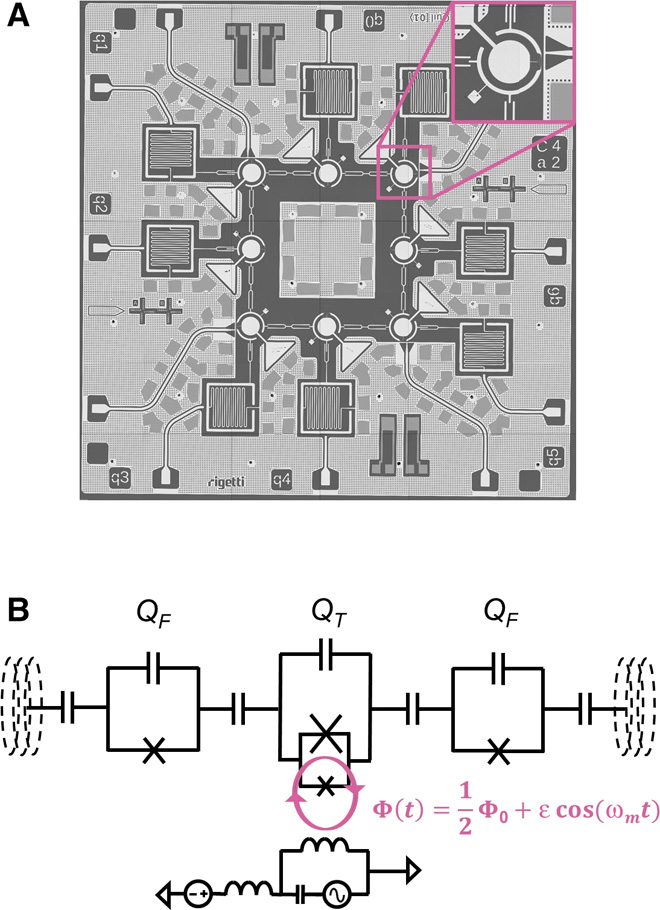
\includegraphics[width=0.8\textwidth]{images/rigetti.jpeg}
        \caption{Rigetti Superconducting Qubits}
    \end{figure}
\end{frame}

\begin{frame}{Superconducting Qubits}
    \begin{columns}
        \column{0.35\textwidth}
        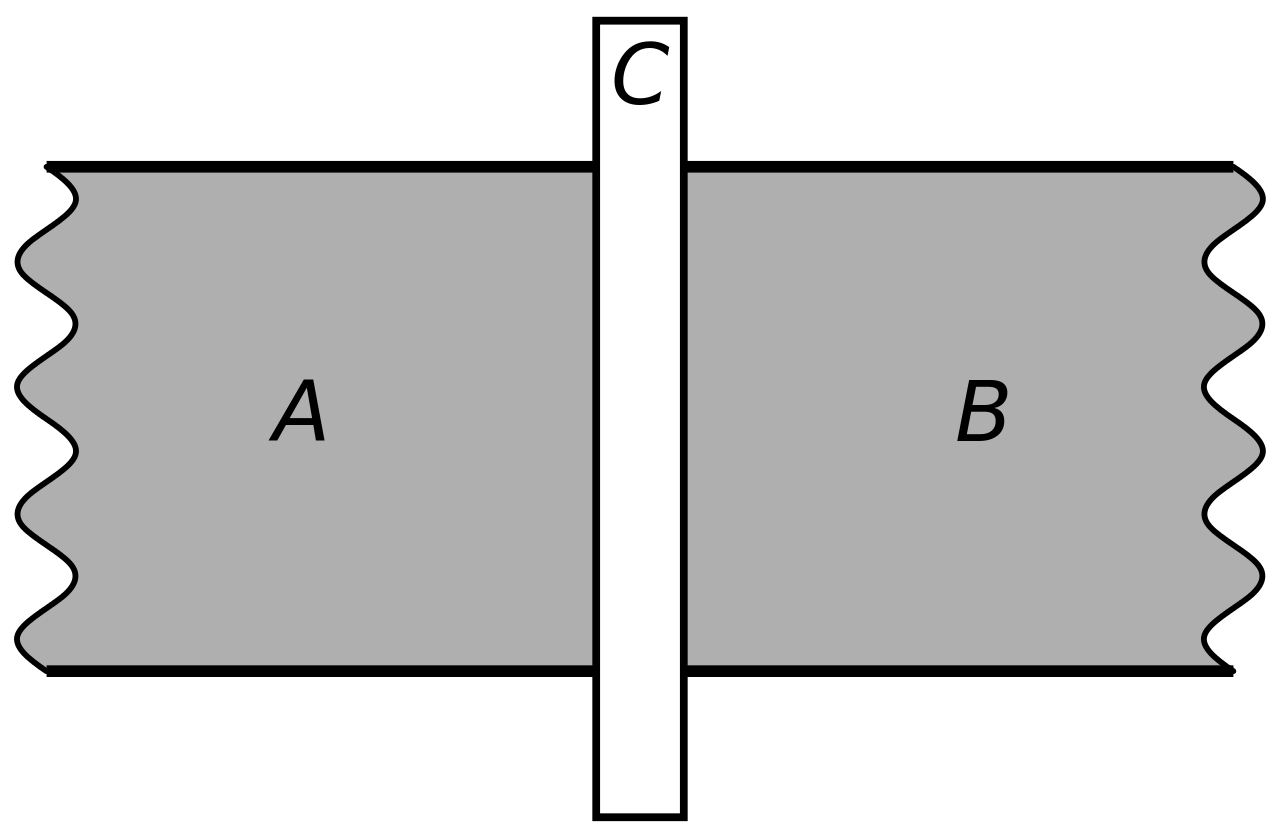
\includegraphics[width=\columnwidth]{images/Single_josephson_junction.svg.png}
        \column{0.65\textwidth}
        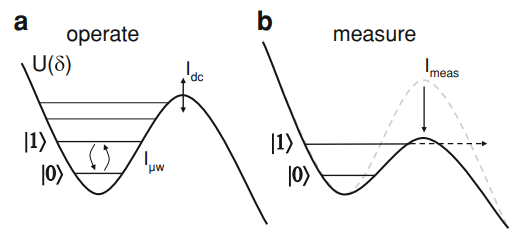
\includegraphics[width=\columnwidth]{images/phase_qubit.png}

    \end{columns}
\end{frame}
    
\begin{frame}{Superconducting Qubits: Gates}
The $R_x$ and $R_y$ gates are used for single qubit operations.\vfill
    \begin{columns}
        \column{0.5\textwidth}
        \centering
        \begin{math}
        R_{X} =
            \begin{pmatrix}
                \cos{\frac{\theta}{2}} & -i\sin{\frac{\theta}{2}} \\ -i\sin{\frac{\theta}{2}} & \cos{\frac{\theta}{2}}
            \end{pmatrix}
        \end{math}\vfill
        \column{0.5\textwidth}
        \centering
        \begin{math}
        R_{Y} =
            \begin{pmatrix}
                \cos{\frac{\theta}{2}} & -\sin{\frac{\theta}{2}} \\ \sin{\frac{\theta}{2}} & \cos{\frac{\theta}{2}}
            \end{pmatrix}
        \end{math}\vfill
    \end{columns}\vfill
    \centering
    The Controlled-Z $CZ$ gate is used for entangling qubits.\vfill
    \begin{math}
        CZ = \begin{pmatrix}
            1 & 0 & 0 & 0\\
            0 & 1 & 0 & 0\\
            0 & 0 & 1 & 0\\
            0 & 0 & 0 & -1\\
        \end{pmatrix}
    \end{math}
\end{frame}



%%%%%%%%%%%%%%%%%%%%%%%%%%%%%%%%%%%%%%%%%%%%%%%%%%%%%%%
% \begin{frame}{QFT}
%     The Fourier Transform is a way of finding out which component
% \end{frame}

\begin{frame}{QPE}
    The Quantum Phase Estimator is a way of working out the energy of each state of a system.
    \vfill
    \centering
    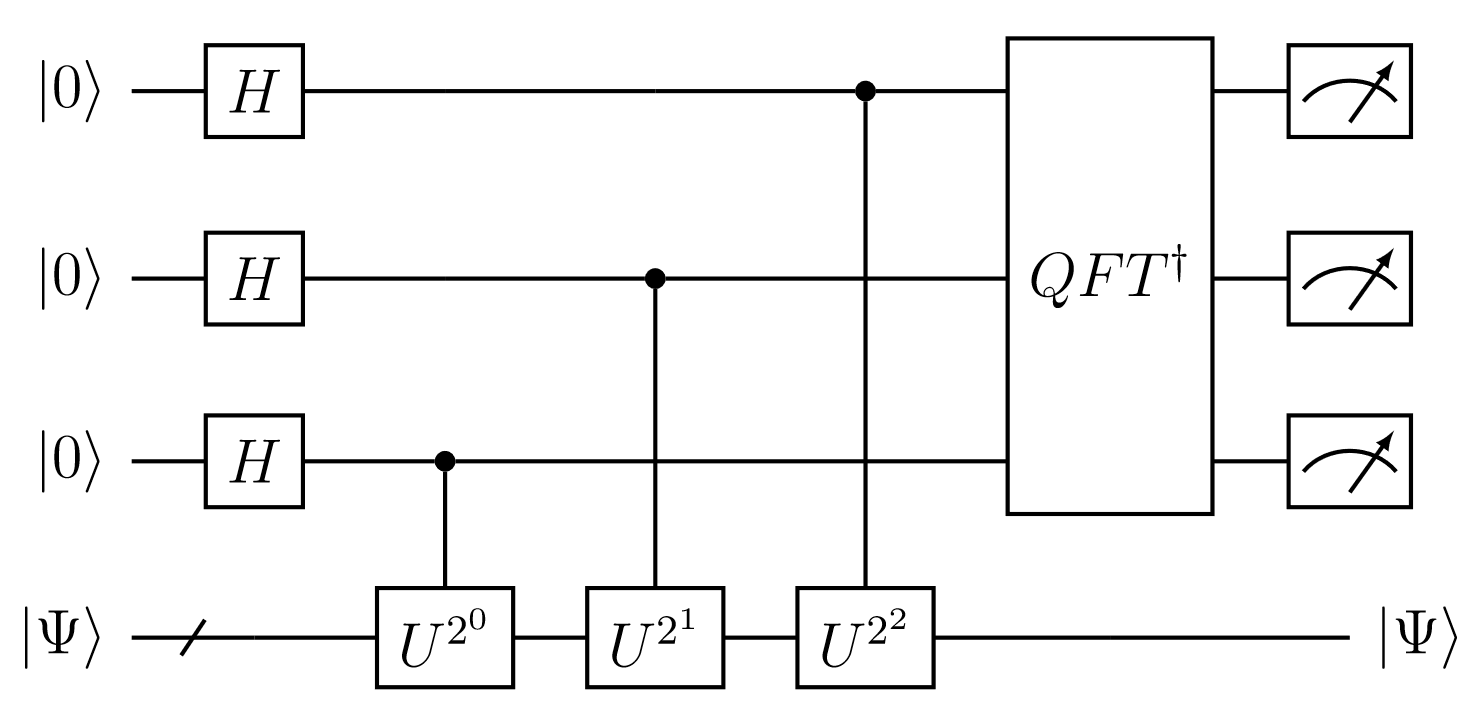
\includegraphics[width=\textwidth]{images/QPE.png}
\end{frame}

\begin{frame}{Iterative QPE}
    We can reduce the number of qubits we need by only using one extra at a time.\vfill
    However, the circuit depth increases.
    \vfill
    \centering
    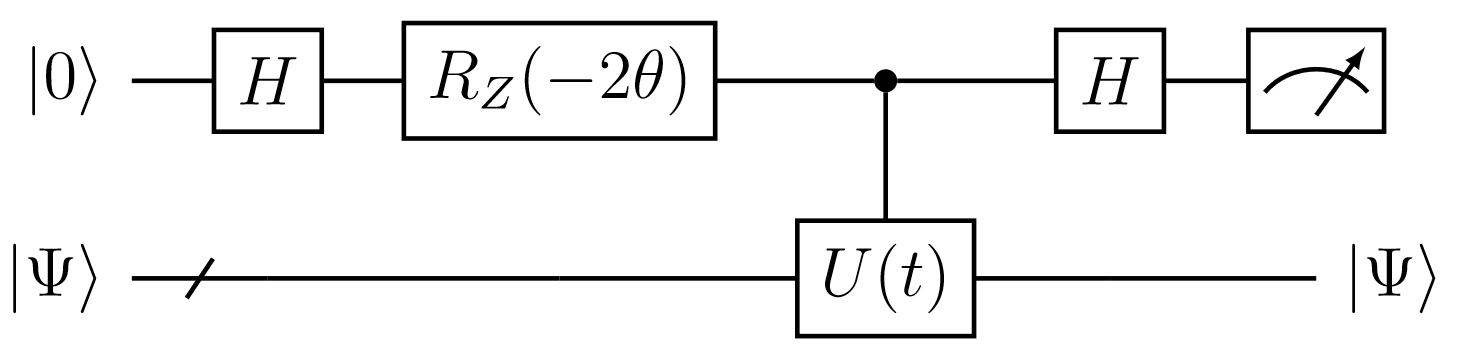
\includegraphics[width=\textwidth]{images/iQPE.png}
\end{frame}

\begin{frame}{NISQ}
    Current quantum computers are very limited in qubit count and depth.\vfill

    We therefore need to design algorithms for the \textbf{N}oisy \textbf{I}ntermidate \textbf{S}mall \textbf{Q}uantum Computers.
    \vfill
    Most algorithm research conducted today is focused on NISQ applications.
\end{frame}

\begin{frame}<1>[label=vqe]{VQE}
    The Variational Quantum Eigensolver is a way to get the lowest energy state $\ket{\psi_0}$ of a system $\ket{\Psi}$.\vfill
    \begin{enumerate}
        \item<1->Initial state input $\ket{\Phi}$
        \pause
        \item<2-> State evolves according to parameterised circuit $\hat{U}(\vec{\alpha})\ket{\Phi} = \ket{\Psi(\vec{\alpha})}$
        \only<2>{
        \begin{center}
            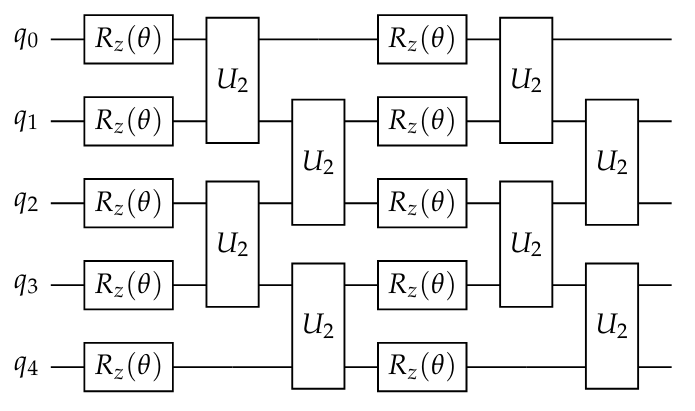
\includegraphics[width=0.6\textwidth]{images/U2ansatz.png}
        \end{center}
        }
        \pause
        \item<3->Measure the energy of the state $E=\bra{\Psi(\alpha)}\hat{H}\ket{\Psi(\alpha)}$
        \pause
        \item<4->Update the parameters $\vec{\alpha}$
        \pause
        \item<5->Repeat Steps 1-3 until we find the minimum energy.
    \end{enumerate}\vfill
    \pause
    Once we've stopped the procedure, we know that $\ket{\Psi_0} = \ket{\Psi(\alpha)}$

\end{frame}
\againframe<2>{vqe}
\againframe<3>{vqe}
\againframe{p1}

\begin{frame}{Variational Principle}
    The variational principal says that we can find the ground state $\ket{\Psi_0}$ by finding a minimum in the energy of parameterised states.\vfill
    \centering
    \begin{math}
        E = \bra{\Psi(\alpha)}\hat{H}\ket{\Psi(\alpha)}
    \end{math}
    \vfill
    \begin{math}
        E_0 \le \bra{\Psi(\alpha)}\hat{H}\ket{\Psi(\alpha)}
    \end{math}
    \vfill
    $\ket{\Psi(\alpha)}$ is the ground state $\ket{\Psi_0}$ when we find a minimum in E!
\end{frame}

\againframe<4>{vqe}
\againframe<5>{vqe}

\begin{frame}{VQE Pros \& Cons}
    \begin{columns}
        \column{0.5\textwidth}
        \begin{itemize}
            \item Reduces circuit depth.
            \item Doesn't need any ancilla qubits
            \item Classical methods for initial state
            \item Finds real $E_0$
            \item Resistant to noise
        \end{itemize}
        \column{0.5\textwidth}
        \begin{itemize}
            \pause
            \item Need to run lots of circuits
            \item Might not be able to update parameters
            \item Global or local minimum?
        \end{itemize}
    \end{columns}
\end{frame}

%%%%%%%%%%%%%%%%%%%%%%%%%%%%%%%%%%%%%%%%%%%%%%%%%%%%%%%
\section{Compilers}
\begin{frame}{Why we need compilers}
We can write circuits using lots of languages.\\\vfill
\pause
Real devices are limited in qubit count and connectivity.\vfill
\pause
We want to run algorithms efficiently.\vfill
\pause
\end{frame}

\begin{frame}[label=compiler]{Compiler Flow}
\label{compiler}
\centering
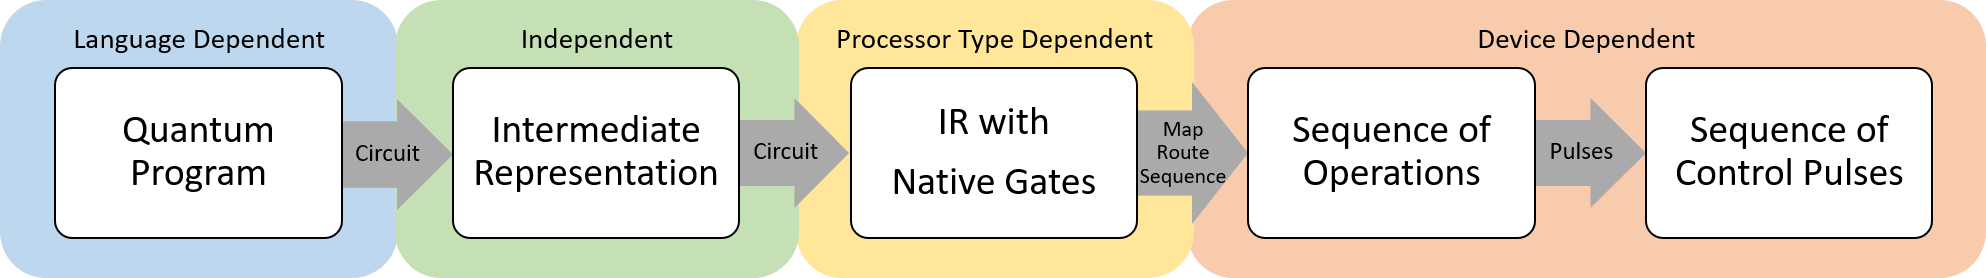
\includegraphics[width=\textwidth]{images/Flow-diagram-colours2.png}
\end{frame}

\begin{frame}{Redundant Gates}
    We might inadvertently write a circuit with gates that cancel out.\\
    Compilers remove these using templates.\\
    \centering
    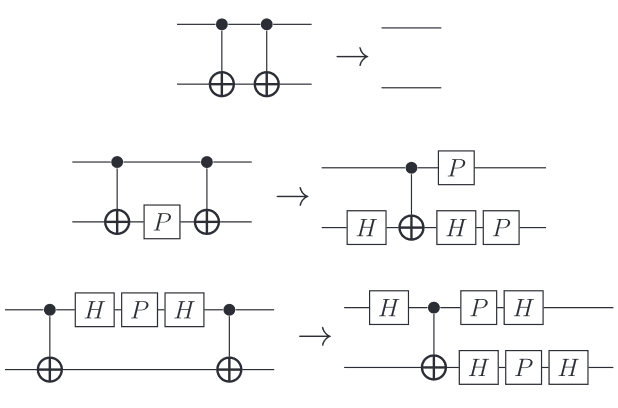
\includegraphics[width=0.8\textwidth]{images/circuit templates.png}
\end{frame}

\begin{frame}<1>[label=ir]{Intermediate Representation}
    \begin{columns}
        \column{0.5\textwidth}
        \centering
        \only<1>{Programming languages output circuits in a standard format called an \textbf{Intermediate Representation}.}
        \only<2>{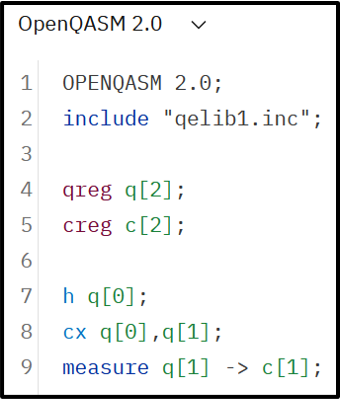
\includegraphics[width=0.8\columnwidth]{images/OpenQASM.png}}
        \column{0.5\textwidth}
        \centering
            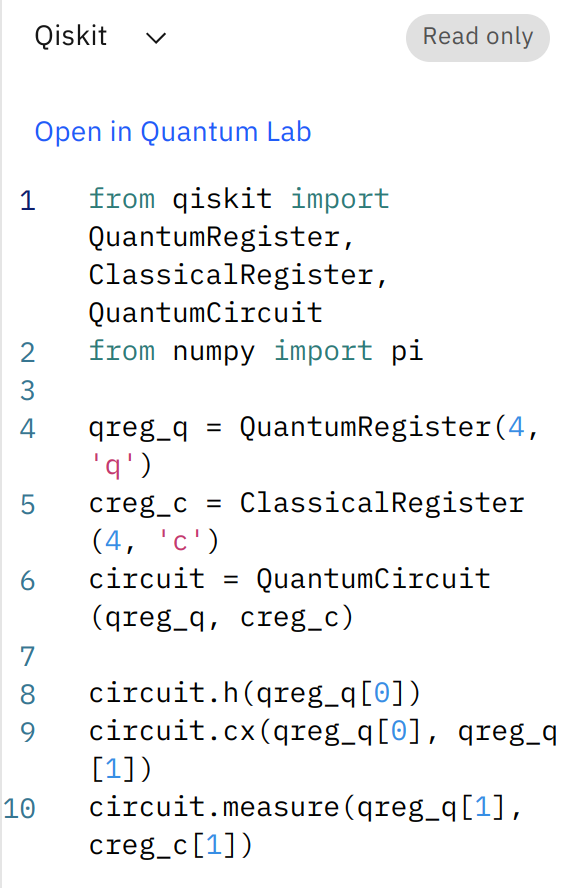
\includegraphics[width=0.8\columnwidth]{images/qiskit_snippet.png}
    \end{columns}
\end{frame}

\againframe<2>{ir}

\begin{frame}{Native Gates}
    \begin{columns}
        \column{0.5\textwidth}
        \textbf{Trapped Ion (IONQ)}\vfill
        \begin{itemize}
            \item GPi
            \item GPi2
            \item Molmer-Sorensen
        \end{itemize}
        \column{0.5\textwidth}
        \textbf{Super Conductor (Rigetti)}\vfill
        \begin{itemize}
            \item Rx
            \item Ry
            \item CZ
        \end{itemize}
    \end{columns}
\end{frame}

\againframe{compiler}

\begin{frame}{Equivalent Circuits}
    \begin{columns}
        \column{0.3\textwidth}
        \centering
            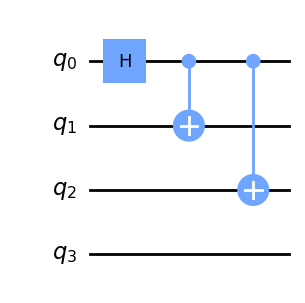
\includegraphics[width=\columnwidth]{images/circ1.png}
        \column{0.3\textwidth}
        \centering
        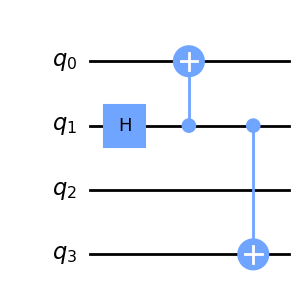
\includegraphics[width=\columnwidth]{images/circ2.png}
        \column{0.3\textwidth}
        \pause
        \centering
        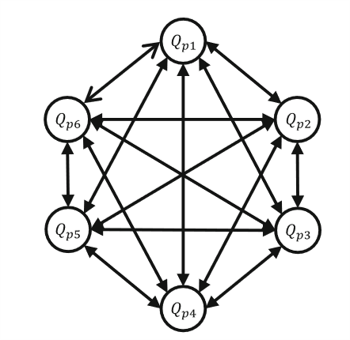
\includegraphics[width=\columnwidth]{images/algoqubits.png}
    \end{columns}
\end{frame}

\begin{frame}{Connectivity}
    \begin{columns}
        \column{0.5\textwidth}
        \begin{figure}
            \centering
            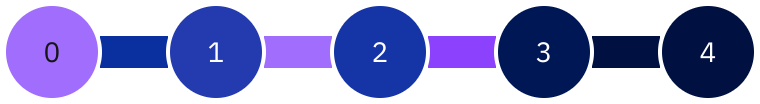
\includegraphics[width=\columnwidth]{images/ibmq_manila_calibrations_readout_error_cx_map_2023-07-14T13_34_25Z.png}
            \caption{Qubit map for IBMQ Manilla}
        \end{figure}
        \column{0.5\textwidth}
        \begin{figure}
            \centering
            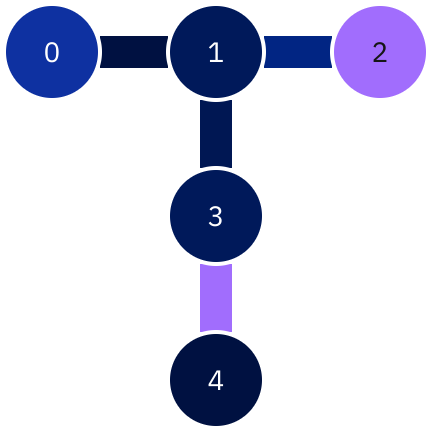
\includegraphics[width=0.7\columnwidth]{images/ibmq_quito_calibrations_readout_error_cx_map_2023-07-10T10_21_51Z.png}
            \caption{Qubit map for IBMQ Quito}
        \end{figure}
    \end{columns}
\end{frame}

\begin{frame}{Quality}
    \begin{columns}
        \column{0.5\textwidth}
        \begin{figure}
            \centering
            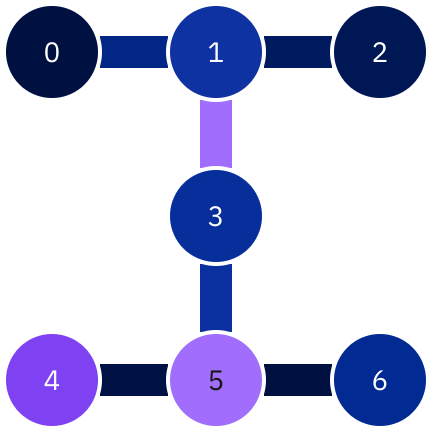
\includegraphics[width=0.7\columnwidth]{images/ibm_lagos_calibrations_readout_error_cx_map_2023-07-14T14_39_24Z.png}
            \caption{Qubit map for IBMQ Lagos}
            \label{fig:lagos}
        \end{figure}
        \column{0.5\textwidth}
        \begin{figure}
            \centering
            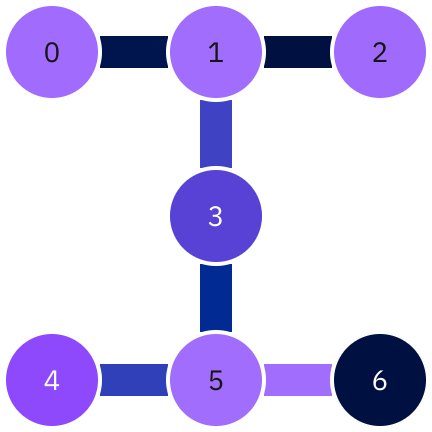
\includegraphics[width=0.7\columnwidth]{images/ibm_perth_calibrations_readout_error_cx_map_2023-07-14T14_39_08Z.png}
            \caption{Qubit map for IBMQ Perth}
            \label{fig:quito}
        \end{figure}
    \end{columns}
\end{frame}

\againframe{compiler}

\begin{frame}{Crosstalk}
    Crosstalk occurs when we apply two gates at once, causing the signals to interfere.
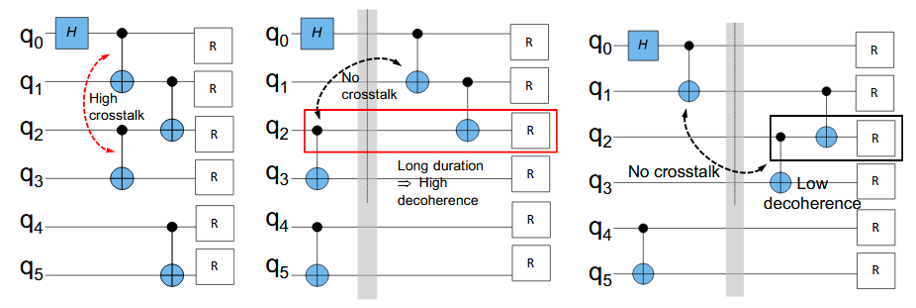
\includegraphics[width=\textwidth]{images/sequence.png}
\end{frame}


%%%%%%%%%%%%%%%%%%%%%%%%%%%%%%%%%%%%%%%%%%%%%%%%%%%%%%%
\section*{What we didn't cover}

\begin{frame}{What we didn't cover}
    \begin{itemize}
        \item Adiabatic Quantum Computing
        \item Non-reversible computing
        \item Braiding
        \item Error Correction
        \item Algorithms
    \end{itemize}
\end{frame}

\begin{frame}{Further Reading}
    \begin{itemize}
        \item IMBQ Textbook
        \item Feynman Lectures
        \item Neilsen \& Chuang
    \end{itemize}
    
\end{frame}

\end{document}